% !TEX root = machine_learning.tex
\chapter{Generalization Bounds}
\label{chap:ms}

We provide, in this chapter, an introduction to some theoretical aspects of  statistical (or machine) learning, mostly focusing on the derivation of ``generalization bounds'' that provide high-probability guarantees on the generalization error of predictors using training data. While these bounds are not always of practical  use, because  making them small
in realistic situations would require an enormous amount of training
data, their derivations and the form they take for specific model classes bring important insight on the structure of the learning problem, and help understand why some methods may perform well while others do not. 

\section{Notation}

We here recall some notation  introduced in \cref{chap:general}. We consider a pair of random variables $(X,Y)$, with $X:\Om\to\CR_X$ and $Y:\Om \to \CG$. Regression problems correspond to $\CR_Y = \mR$ (or $\mR^q$ if multivariate) and classification to $\CR_Y$ being a finite set. A predictor is a function $f: \CR_X\to\CR_Y$. The general prediction problem is to find such a predictor within a class of functions, denoted $\CF$, minimizing the prediction (or generalization error)
\[
R(f) = \myE(r(Y, f(X)))
\]
where $r: \CR_Y\times\CR_Y \to [0. +\infty)$ is a risk function. 

A training set is a family $T = ((x_1, y_1), \ldots, (x_N, y_N)) \in (\CR_X\times \CR_Y)^N$, the set $\CT$ of all possible training sets  therefore being the set of all finite sequences in $\CR_X\times \CR_Y$. A training algorithm can then be seen as a function $\CA: \CT \to \CF$ which associates to each training set $T$ a function $\CA(T) = \hat f_T$. 
\bigskip

Given $T \in \CT$, The training set error associated to a function $f\in \CF$ is
\[
\hat R_T(f) = \frac{1}{|T|} \sum_{(x,y)\in T} r(y, f(x)))
\]
and the in-sample error associated to a learning algorithm is the function $T \mapsto \CE_T \defeq \hat R_T(\hat f_T)$.  Fixing the size ($N$) of $T$, one also considers the random variable $\mathbb T$ with values in $\CT$ distributed as an $N$-sample of the distribution of $(X,Y)$. 

A good learning algorithm should be such that the generalization error $R(\hat f_T)$ is small, at least in average (i.e., $E(R(\hf_{\mathbb T}))$ is small). Our main goal in this chapter is to describe generalization bounds trying to find upper-bounds for $R(\hat f_T)$ based on $\CE_T$ and properties of the function class $\CF$. These bounds will reflect the bias-variance trade-off, in that, even though large function classes provide smaller in-sample errors, they will also induce a large additive term in the upper-bound, accounting for the ``variance'' associated to the class. 

\begin{remark}
Both variables $X$ and $Y$ are assumed to be random in the previous setting,
but there are often situations when one of them is ``more random'' than the
other. Randomness in $Y$ is associated to measurement errors, or
ambiguity in the decision.  Randomness in $X$ more generally relates to
the issue of sampling a dataset in a large dimensional space. In some
cases, $Y$ is not random at all: for example, in object recognition,
the question of assigning categories for images such as those depicted in  \cref{fig:pipe} has a quasi-deterministic answer. Sometimes, it is $X$ who is not random, for example when observing noisy signals where $X$ is a deterministic discretization of a time interval and $Y$ is some function of $X$ perturbed by noise.  
\end{remark}

\begin{figure}
\centering
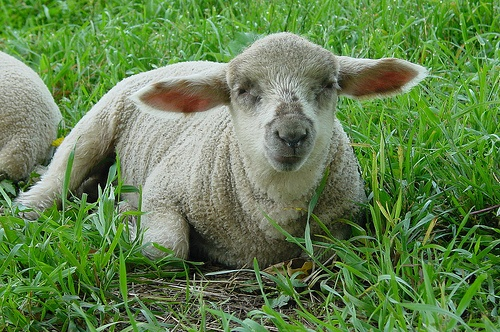
\includegraphics[width=0.4\textwidth]{Figures/2007_000175.jpg}
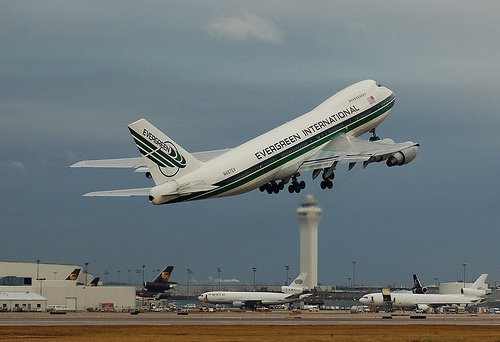
\includegraphics[width=0.4\textwidth]{Figures/2007_001288.jpg}\\

\includegraphics[width=0.4\textwidth]{Figures/2007_000876.jpg}

\includegraphics[width=0.4\textwidth]{Figures/2007_002227.jpg}
\caption{\label{fig:pipe} Images extracted from the PASCAL challenge 2007 dataset \citep{everingham2010pascal}, in which categories must be associated with images. There is little ambiguity on correct answers  based on observing the image, i.e., little randomness in the variable $Y$.}
\end{figure}



\section{Penalty-based Methods and Minimum Description Length}
\label{sec:is.err}

\subsection{Akaike's information criterion}

%Sometimes, $X$ is small dimensional and densely sampled, but $Y$ is subject to noise. The following discussion is well adapted to such cases, since it focuses the generalization error only on the output component.



We make a computation under the following assumptions. We assume a regression model $Y = f_\theta(X) + \ep$ where $\epsilon \sim \CN(0, \sigma^2)$ and $f$ is some function parametrized by $\theta \in \mR^m$. We also assume that the true distribution is actually covered by this model and represented by a parameter $\theta_0$. Let $\hth_T$ denote the parameter estimated by least squares using a training set $T$, and denote for short $\hf_T = f_{\hth_T}$. 

The in-sample error is
\[
\CE_T = \frac1N \sum_{k=1}^N (y_k - \hf_T(x_k))^2.
\]
We  want to compare the training-set-averaged prediction error and the average in-sample error, namely compute the error bias
\[
\Delta_N = \myE(R(f_\mT)) - \myE(\CE_\mT)\,.
\]
%Recall that we are working under the assumption that the data distribution corresponds to the  model $Y = f_{\th_0}(X) + \epsilon$. 
Write 
\[
\Delta_N = \myE(R(f_\mT)) - R(f_{\th_0}) + R(f_{\th_0}) - E(\CE_\mT).
\]

We  make a heuristic argument to evaluate $\Delta_N$.
We can use the fact that $\hth_T$ minimizes the empirical error and write
\[
\frac1N \sum_{k=1}^N (Y_k-f_{\th_0}(X_k))^2 = \CE_\mT +  \sigma^2 (\hth_\mT - \th_0)^T J_{\mT} (\hth_\mT - \th_0) + o(|\hth_\mT - \th_0|^2)
\]
with 
\[
J_T = \frac1{2\sigma^2 N} \sum_{k=1}^N \prt_\th^2 ((y_k - f_\th(x_k))^2)_{|_{\th-\hth_T}},
\]
which is an $m$ by $m$ symmetric matrix.

Now, using the fact that $\th_0$ minimizes the mean square error (since $f_{\th_0}(x) = \myE(Y|X=x)$), we can write, for any $T$:
\[
R(f_T) = R(f_{\th_0}) +  \sigma^2 (\hth_T - \th_0)^T I  (\hth_T - \th_0) + o(|\hth_T - \th_0|^2)
\]
with 
\[
I = \frac1{2\sigma^2}  \myE(\prt_\th^2 (Y-f_{\th}(X))^2_{|_{\th-\th_0}}).
\]

As a consequence, we can write (taking expectations in both Taylor expansions)
\[
\Delta_N = \sigma^2 \myE \left((\hth_\mT - \th_0)^T J_{\mT} (\hth_\mT - \th_0) \right)+ \sigma^2 \myE\left((\hth_\mT - \th_0)^T I  (\hth_\mT - \th_0)\right) + o(\myE(|\hth_\mT - \th_0|^2)).
\]
(We skip hypotheses and justification for the analysis of the residual term.)

We now note that, because we are assuming a Gaussian noise, and that the true data distribution belongs to the parametrized family, the least-square estimator is also a maximum likelihood estimator. Indeed, the likelihood of the data is
\[
\frac{1}{(2\pi\sigma^2)^{N/2}} \exp\left(- \frac1{2\sigma^2}\sum_{k=1}^N (Y_k - f_{\th}(X_k))^2\right) \prod_{k=1}^N \phi_X(X_k)
\]
where $\phi_X$ is the p.d.f.  of $X$ and does not depend on the unknown parameter. 

We can therefore apply classical  results from mathematical statistics \citep{van2000asymptotic}. Under some mild smoothness assumptions on the mapping $\th \mapsto f_{\th}$,  $\hth_\mT$ converges to $\th_0$ in probability when $N$ tends to infinity, the matrix $J_\mT$ converges to $I$, which is the model's Fisher information matrix, and $\sqrt N (\hth_\mT - \th_0)$ converges in distribution to a Gaussian $\CN(0, I^{-1})$ . This implies that both $N(\hth_\mT - \th_0)^T J_{\mT} (\hth_\mT - \th_0)$ and $N(\hth_\mT - \th_0)^T I  (\hth_\mT - \th_0)$ converge to a chi-square distribution with $m$ degrees of freedom, whose expectation is $m$, which indicates that $\Delta_N$ has order $2\sigma^2m/N$.


This analysis can be used to develop model selection rules, in which one chooses between models of dimensions $k_1 <k_2 < \cdots < k_q = m$ (e.g., by truncating the last coordinates of $X$).  The rule suggested by the previous computation is to  select $j$ minimizing  
\[
\CE^{(j)}_T(\hf_T) + \frac{2\sig^2 k_j}N,
\]
  where $\CE^{(j)}$ is the in-sample error computed using the $k_j$-dimensional model.
This is an example of a penalty-based method, using the so-called Akaike's
information criterion (AIC) \citep{akaike1973information}. 


\subsection{Bayesian information criterion and minimum description length}
Other penalty-based methods are more size-averse and replace  the
constant, $2$, in AIC by  a function of $N = |T|$, for example
$\log N$. Such a change can be justified by a Bayesian
analysis, yielding the Bayesian information criterion (BIC) \citep{schwarz1978estimating}. The approach in this case is not based on an evaluation of the error, but on an asymptotic estimation of the posterior distribution resulting from a Bayesian model selection principle.  Like in the previous section, we content ourselves with a heuristic discussion.


Let us consider a statistical model parametrized by $\th\in \Th$, where $\Th$ is an open convex subset of $\mR^m$ with p.d.f. given by
\[
f(z;\theta) = \exp(\theta^TU(z) - C(\th))\,,
\]
with $U: \mR^d \to \mR^m$and $z = (x,y)$. We are given a family of sub-models represented by $\CM_1, \ldots, \CM_q$, where, for each $j$, $\CM_j$ is the intersection of $\Theta$ with a $k_j$-dimensional affine subspace of $\mR^m$. We are also given a prior distribution for $\th$ in which a sub-model is first chosen, with probabilities $\al_1, \ldots, \al_q$, and given that, say, $\CM_j$ is selected, $\th\in \CM_j$ is chosen with a probability distribution with density $\phi_j$ with respect to Lebesgue's measure on $\CM_j$ (denoted $dm_j$). Given training data $T = (z_1, \ldots, z_N)$, Bayesian model selection consists in choosing the model $\CM_j$ where $j$ maximizes the posterior log-likelihood
\[
\mu(\CM_j|T) = \log\int_{\mR^m} \al_j e^{N(\th^T \bar U_T - C(\th))} \phi_j dm_j(\th)
\]
where $\bar U_T = (U(z_1) + \cdots + U(z_N))/N$. 

Consider the maximum likelihood estimator $\hat \th_j$ within  $\CM_j$, maximizing $\ell(\theta, \bar U_T) = \th^T \bar U_T - C(\th)$ over $\CM_j$. Then one has
\[
\ell(\th, \bar U_T) = \ell(\hat\th_j, \bar U_T) + \frac12 (\th - \hat \th_j)^T \prt^2_\th\ell(\hth_j, \bar U_T)(\th-\hth_j) + R_j(\th, \hth_j) |\th-\hth_j|^3
\]
Note that the first derivative of $\ell$ is $\prt_\th \ell  = \bar U - E_\th(U)$ where $E_\th$ is the expectation for $f(\cdot, \th)$. The second derivative is $-\var_\th(U)$ (showing that $\ell$ is concave) and the third derivative involves third-order moments of $U$ for $E_\th$ and (like the second derivative) does not depend on $\bar U_T$. In particular, we can assume that, for any $M>0$, there exists a constant $C_M$ such  that whenever $\max(|\th|, |\hth_j|) \leq M$, we have $R_j(\th, \hth_j) \leq C_M$.

The law of large numbers implies that $\bar U_T$ converges to a limit when $N$ tends to infinity, and our assumptions imply that $\hth_j$ converges to the parameter providing the best approximation of the distribution of $Z$ for the Kullback-Leibler divergence. In particular, with probability 1, there exists an $N$ such that $\hth_j$ belongs to any large enough, but fixed, compact set. Moreover, the second derivative $\ell(\hth_j)$ will also converge to a limit, $-\Sig_j$. 

For any $\ep>0$, write
\begin{multline*}
\int_{\mR^m} \al_j e^{N(\th^T \bar U_T - C(\th))} \phi_j dm_j(\th) \\
= \int_{|\th - \hth_j| \leq \ep} e^{N(\th^T \bar U_T - C(\th))} \phi_j dm_j(\th) + \int_{|\th - \hth_j| \geq \ep} e^{N(\th^T \bar U_T - C(\th))} \phi_j dm_j(\th)\,.
\end{multline*}
The second integral  converges to $0$ exponentially fast when $N$ tends to $\infty$. The first one  behaves essentially like 
\[
\int_{\CM_j} e^{- \frac12 N (\th - \hat \th_j)^T \Sig_j^{-1} (\th - \hat \th_j) + \log\phi_j(\th)} dm_j(\th)\,.
\]
Neglecting $\log\phi_j(\th)$, this integral behaves like $(2\pi\det (\Sig_j/N))^{-1/2}$, whose logarithm is $(-k_j(\log N)/2)$ plus constant terms. As a consequence, we find that 
\[
\mu(\CM_j\mid T) = \max_{\th\in \CM_j} \ell(\th) - \frac {k_j}2 \log N + \text{ bounded terms}.
\]


Consider, as an example, linear regression  with $Y = \be_0 + b^T x + \sig^2 \nu$ where $\nu$ is a standard Gaussian random variable. Assume that the distribution of $X$ is known, or, preferably, make the previous discussion conditional to $X_1, \ldots, X_N$. 
Let sub-models $\CM_j$ correspond to the assumption that all but the first $k_j-1$ coefficients of $b$ vanish. 
Then, up to bounded terms, the Bayesian estimator must minimize (over such parameters $b$)
\[
\frac1{2\sig^2} \sum_{k=1}^N (y_k - \be_0 - b^T x_k)^2 + \frac {k_j} 2 \log N\,.
\]
or
\[
\CE^{(j)}_T + \frac{k_j\sig^2}N \log N\,.
\]


\bigskip
We now turn to another
interesting point of view, which provides the same penalty, based
on maximum description length principle (MDL; \citet{rissanen1989stochastic})  measuring the coding efficiency of a model.

Let us fix some notation. We assume that one has $q$ competing models
for predicting $Y$ from $X$, for example, linear
regression models based on different subsets of the explanatory
variables. Denote these models $\CM_1, \ldots, \CM_q$. Each model will
be seen, not as an assumption on the true joint distribution of $X$ and
$Y$, but rather as a tool to efficiently encode the training set
$((x_1, y_1), \ldots, (x_N, y_N))$. To describe MDL, which selects the model that provides the most efficient code, we need to
reintroduce a few basic concepts of information theory.

The entropy of a discrete probability $P$ over a set $\Om$ is 
$$
\CH_2(P) = - \sum_{x\in \Om} p_x \log_2p_x.
$$
(The logarithm in base 2 is used because of the tradition of coding with
bits in information theory.)

For a discrete random variable $X$, the entropy $\CH_2(X)$ is $\CH_2(P_X)$
where $P_X$ is the probability distribution of $X$. The relation
between the entropy and coding theory is as follows: a code is a
function which associates to any element $\om\in \Om$ a string of bits
$c(\om)$. The associated code-length is denoted $l_c(\om)$, which is simply
the number of bits in $c(\om)$. When $P$ is a probability on $\Om$,
the efficiency of a code is measured by the average code-length:
$$
E_P(l_c) = \sum_{\om\in\Om} l_c(\om) P(\om).
$$

Shannon's theorem \citep{shannon1948mathematical, cover2012elements} states that, under some conditions on the code
(ensuring that any sequence of words can be recognized as soon as it is observed: one says that it is instantaneously decodable) the average
code length can never be larger than the entropy of $P$. Moreover, it states that
there exists codes that achieve this lower bound with no more than one
bit loss,  such that for all $\om$, $l_c(\om) \leq -
\log_2(P(\om)) + 1$. These optimal codes, such as the Huffman code \citep{cover2012elements}, can completely be determined from the
knowledge of $P$. This allows one to interpret a probability $P$ on $\Om$
as a tool for designing codes with code-lengths essentially equal to   ($-\log_2
P$).

This statement can be generalized to continuous random
variables (replacing the discrete probability $P$ by a probability density function, say $\phi$) if one introduces a coding precision level, denoted $\de_0$, meaning that the decoded values may differ by no more than $\de_0$ from the encoded ones. The result is that
the optimal code-length at precision $\de_0$ can be estimated (up to one extra bit) by $- \log_2 \phi - \log_2\de_0$. 

In our context, each model of the conditional distribution of $Y$ given $X$, with conditional density 
 $\phi(y|x)$, provides a way to encode the training
set with a total code length, for $(y_1, \ldots, y_N)$, of
$$
- \sum_{k=1}^N \log_2 \phi(y_k\mid x_k) - N\log_2\de_0
$$
(working, as before, conditionally to $x_1, \ldots, x_N$).
We assume that the precision at which the data is encoded is fixed,
which implies 
that the last term does not affect the model choice. Now, assume a sequence of $m$  parametrized model classes, $\CM_1, \ldots, \CM_m$ and let $\phi(y\mid x,\th, \CM_j)$ denote the conditional distribution with parameter $\th$ in the class $\CM_j$. 
Within model $\CM_j$, the optimal code length corresponds to the
maximum likelihood:
$$
- \sum_{k=1}^N \log_2 \phi(x, y\mid \hat \th_j, \CM_j) = - \max_{\th}\left(\sum_{k=1}^N \log_2 \phi(x, y; \th, \CM_j)\right).
$$

If the models are nested, which is often the case,  the most efficient  will always be the
largest model, since the maximization is on a larger set. However,  the minimum description length (MDL) principle uses the fact that, in
order to decode the compressed data, the model, including its optimal
parameters, has to be known, so that the complete code  needs to
include a model description. The decoding algorithm will then
be: decode the model, then use it to decode the data. 

So assume that a model (one of the $\CM_j$'s) has a $k_j$-dimensional
parameter $\th$. Also assume that a probability distribution, $\pi(\th\mid \CM_j)$, is used to
encode $\th$. Also choose a precision level, $\de_{ij}$, for each coordinate in
$\th$, $i=1, \ldots, k_j$. (Previously, we could consider the precision of
the $y_k$, $\de_0$, as fixed, but now, the precision level for parameters is a variable that will be optimized.) The total description length using this model now becomes
$$
- \sum_{k=1}^N \log_2 \phi(y_k\mid x_k; \th, \CM_j) - \log_2\pi(\th\mid \CM_j) -
\sum_{i=1}^{k_j} \log_2(\de_{ij}).
$$

Let $\hth^{(j)}$ be the parameter that maximizes
$$
L(\th\mid \CM_j)  = \sum_{k=1}^N \log_2 \phi(y_k\mid x_k; \th, \CM_j) + \log_2\pi(\th\mid \CM_j)$$ 

If $\pi$ is interpreted as a prior distribution of the parameters,
$\hth^{(j)}$ is the {\em maximum a posteriori} Bayes estimator. We now take
the correction caused by 
$(\de_{ij}, i=1, \ldots, k_j)$ into account, by assuming that the $i$th coordinate in $\hth^{(j)}$
is truncated to  $-\log_2 \de_i$ bits. Let
$\bth^{(j)}$ denote this approximation. A second-order expansion of
$L(\th|\CM_j)$ around $\hth^{(j)}$ yields (assuming sufficient differentiability) 
$$
L(\bth^{(j)}\mid \CM_j) = L(\hth^{(j)}\mid \CM_j) + \frac{1}{2} (\bth^{(j)} - \hth^{(j)})^T S_{\hth^{(j)}}
(\bth^{(j)} - \hth^{(j)}) + o(|\bth^{(j)}- \hth^{(j)}|^2)
$$
where $S_\th$ is the matrix of second derivatives of  $L(\cdot\mid \CM_j)$ at
$\th$. Approximating $\bth^{(j)} - \hth^{(j)}$ by $\de^{(j)}$ (the
$k_j$-dimensional vector with coordinates $\de_{ij}$, $i=1, \ldots, k_j$), we see that the precision
should maximize
$$
\frac{1}{2} (\de^{(j)})^T S_{\hth^{(j)}} \de^{(j)} + \sum_{i=1}^{k_j} \log_2\de_{ij}.
$$
Note that $S_{\hth^{(j)}}$ must be negative semi-definite, since $\hth$ is a
local maximum. Assuming it is non-singular, the previous
expression can be maximized and yields
\begin{equation}
\label{max.riss}
S_{\hth^{(j)}} \de^{(j)} = -\frac{1}{\log 2} \frac{1}{\de^{(j)}}
\end{equation}
where $1/\de^{(j)}$ is the vector with coordinates $(1/\de_{ij})$.

Let us now make an asymptotic evaluation. Because  $L(\th\mid \CM_j)$
includes a sum over $N$ independent terms, it is reasonable to assume that $S_{\hth^{(j)}}$ has order
$N$, and more precisely, that $S_{\hth^{(j)}}/N$ has a limit. Rewrite
 \cref{max.riss} as
$$
\frac{S_{\hth^{(j)}}}{N} {\sqrt{N}\de^{(j)}} = -\frac{1}{\log 2} \frac{1}{\sqrt{N}\de^{(j)}}\,.
$$
This implies that $\sqrt{N}\de^{(j)}$ is the solution of an equation which
stabilizes with $N$, and it is therefore reasonable to assume that the optimal $\de_{ij}$ takes the form $\de_{ij} =
c_i(N\mid \CM_j)/\sqrt{N}$, with $c_i(N\mid \CM_j)$ converging to some limit when $N$ tends
to infinity. The total cost can therefore be estimated by
$$
- L(\hth^{(j)}\mid \CM_j) + \frac{k_j}{2} \log_2 N - \frac{k_j}{2} - \sum_{i=1}^{k_j} \log_2 c_i(N\mid \CM_j)
$$
The last two terms are O(1), and can be neglected, at least when $N$
is large compared to $k_j$. The final criterion becomes the
penalized likelihood
$$
l_d(\th\mid \CM_j) = L(\th|\CM_j) - \frac{k_j}{2} \log_2 N
$$
in which we see that the dimension of the model appears with a factor
$\log_2N$ as announced (one needs to normalize both terms by $N$ to
compare with the previous paragraph). 

%Ridge regression corresponds to the case when
%$\pi(\th)$ is Gaussian, and the conditional distribution of $y$ given
%$x$ is Gaussian with fixed variance and expectation $\scp{\th}{x}$. The penalty factor, $\log_2 N$,
%in this case, is stronger than the one provided by the AIC criterion,
%in which only a constant appeared in front of $N$ (note however that
%the $\log_2 N$ penalty is generally the one which provides consistent
%asymptotic results: when $N$ is large, the model which is learned is
%the ``true one''). Note that this approach directly applies to
%classification problems, in particular logistic regression where the
%argument carries over without change.


%\section{Generalization Bounds}
\section{Concentration inequalities}
\label{sec:ci}

The discussion of the AIC was a first attempt at evaluating a prediction error.
It was however done under very specific parametric assumptions, including the fact that the true distribution of the data was within the considered model class.
It was, in addition, a bias evaluation, i.e., we estimated how much, in average, the in-sample error was less than the generalization error.
We would like to obtain upper bounds to the generalization error that hold with high probability, and rely as little as possible on assumptions on the true data distribution. 
%Even if, in most instances, the bounds we are going to derive are not really practical, they however provide insight on the structure of the learning problem and help understand why some machine learning methods work or don't.
% help design sensible and efficient model selection methods.

One of the main tools used in this context are concentration inequalities, which provide upper bounds on the various probabilities of events involving a large number of random variables. The current section provides a review of some of these inequalities.
\bigskip

%This section is based on the general presentation of \cite{bbl02}. 
%We restrict, in the following, to two-class classification
%problems: $y\in\CR_Y = \{0,1\}$. We assume that the loss function $L$ is
%bounded by 1, which is the case for the binary one $L(y,y') =
%\chi_{y\neq y'}$.


%\subsubsection{Concentration of the empirical mean}
\subsection{Cram\'er's theorem}
If $X_1, X_2, \ldots$ are independent, integrable random variables with identical distributions (to that of a random variable $X$), the law of large numbers tells us that the empirical mean $\bar X_N = (X_1 + \cdots + X_N)/N$ converges with probability one to $m=E(X)$. When the variables are square integrable, Chebychev's inequality provides an easy proof of the weak  law of large numbers. Indeed,
\[
\myP\big(|\bar X_n - m| > \ep\big) \leq \frac{1}{\ep^2} \myE\big((\bar X_N - m)^2\bfone_{|\bar X_n - m| > \ep}\big) \leq \frac{\mathrm{var}(\bar X_N)}{\ep^2} = \frac{\mathrm{var}(X)}{N\ep^2}.
\]

A stronger assumption on the moments of $X$ yields a stronger inequality. One says that $X$ has exponential moments if there exists $\la_0 > 0$ such that $\myE(e^{\la_0|X|}) < \infty$. In this case, the cumulant-generating function, defined, for $\la\in\mR$, by
\begin{equation}
\label{eq:laplace}
M_X(\la) = \log \myE(e^{\la X}) \in [0, +\infty], 
\end{equation}
is finite for $\la \in [-\la_0, \la_0]$. 

Here are a few straightforward properties of the cumulant-generating function. 
\begin{enumerate}[label=(\roman*)]
\item One has $M_X(0) = 0$. 
\item For any $a\in \mR$, one has
$M_{aX}(\la) = M_X(a\la)$. 
\item If $X_1$ and $X_2$ are independent variables, one also has
\[
M_{X_1+X_2}(\la) = M_{X_1}(\la) + M_{X_2}(\la).
\]
In particular, $M_{X+a}(\la) = M_X(\la) + \la a$, so that $M_{X-E(X)}(\la)  = M_X(\la) - \la E(X)$.
\item
Finally, Markov's inequality (which states that, for any non-negative variable $Y$, $P(Y> t) \leq E(Y)/t$) applied to $Y = e^{\la X}$ for $\la> 0$ yields
\begin{equation}
\label{eq:markov.exp}
\myP(X>t) = \myP(e^{\lambda X} > e^{\lambda t}) \leq e^{M_X(\la) - \la t}\,.
\end{equation}
(Note that this inequality is trivially true for $\lambda=0$.)
\end{enumerate}


From these properties, one can easily derive a concentration inequality for the mean of independent random variables. 
We have $M_{\bar X_N}(\la) = N M_X(\la/N)$ and applying \eqref{eq:markov.exp} we get, for any $\la \geq 0$ and $t>0$
\[
\myP(\bar X_N - m > t) \leq e^{-\la(m+t) + M_{\bar X_N}(\la)} = e^{-N \left(\frac{\la(m+t)}N - M_X\left(\frac{\la}N\right)\right)}
\]
where the right-hand side may be infinite. Because this inequality is true for any $\la$, we have
\[
\myP(\bar X_N - m > t) \leq e^{-N M_{X,+}^*(m+t)}
\]
where $M_{X,+}^*(u) = \sup_{\la\geq 0} (\la u - M_X(\la))$, which is non-negative since the maximized quantity vanishes for $\lambda=0$. A symmetric computation yields   
\[
P(\bar X_N - m < -t) \leq e^{-N M_{X,-}^*(m-t)}
\]
where $M_{X,-}^*(t) = \sup_{\la\leq 0} (\la t - M_X(\la))$, which is also non-negative. 

Let 
\begin{equation}
\label{eq:cramer}
M_X^*(t) = \sup_{\la\in \mR} (\la t - M_X(\la)) \geq 0
\end{equation}
(this is the Fenchel-Legendre transform of the cumulant generating function, sometimes called the Cram\'er transform of $X$). One  has $M_X^*(m+t) = M^*_{X,+}(m+t)$ for $t>0$. Indeed, because $x\mapsto e^{\la x}$ is convex, Jensen's inequality implies that 
\[
\myE(e^{\la X}) \geq e^{\la m}
\]
so that $\la (m+t) - M_X(\la) \leq \la t < 0$ if $\la<0$.  Similarly,  $M_X^*(m-t) = M^*_{X,-}(m-t)$ for $t >0$. We therefore have the following result.
\begin{theorem}
\label{th:cramer.inf}
Let $X_1, \ldots, X_N$ be independent and identically distributed random variables. Assume that these variables are integrable and let $m = \myE(X_1)$. Then, for all $t>0$,
\[
\myP(\bar X_N - m > t) \leq e^{-N M_{X}^*(m+t)}
\]
and
\[
\myP(|\bar X_N - m| > t) \leq 2e^{-N \min(M_X^*(m+t), M_X^*(m-t))}
\]
\end{theorem}
The last inequality derives from
\[
\myP(|\bar X_N - m| > t)  = \myP(\bar X_N - m > t) + \,uP(\bar X_N - m < -t)\,.
\]

This is our first example of concentration inequality that shows that, when 
\[
\min(M_X^*(m+t), M_X^*(m-t))>0,
\]
 the probability of a deviation by $t$ at least of $\bar X_n$ from its mean decays exponentially fast.  The derivation of the inequality above was quite easy: apply Markov's inequality in a parametrized form and optimize over the parameter. It is therefore surprising that this inequality is sharp, in the sense that a similar lower bound also holds. Even though we are not going to use it in the rest of this chapter, it is worth sketching the argument leading to this lower bound, which involves an interesting step making a change of measure. 

Assume (without loss of generality) that $m=0$ and consider $\myP(\bar X_n > t)$. Assume, to simplify the discussion, that the supremum of $\la \mapsto \ep\la - M_X(\la)$ is attained at some $\la_t$. We have 
\[
\prt_\la M_X(\la) = \frac{\myE(Xe^{\la X})}{\myE(e^{\la X})}.
\]
Let $q_\la(x) = \frac{e^{\la x}}{\myE(e^{\la X})}$ and $\myP_\la$ (with expectation $\myE_\lambda$) the probability distribution on $\Omega$ with density $q_\la(X)$ with respect to $\myP$, so that $\prt_\la M_X(\la) = \myE_\la(X)$. We have, since $\la_t$ is a maximizer, $\myE_{\la_t}(X) = t$. Moreover, fixing $\de >0$, 
\begin{align*}
\myP(\bar X_N > t) &= \myE(\bfone_{\bar X_N > t}) \\
& \geq   \myE(\bfone_{ |\bar X_n - t-\de| < \de}) \\
& \geq  \myE\big(\bfone_{ |\bar X_n - t -\de| < \de} e^{N\la \bar X_N - Nt - 2N\de}\big) \\
& = e^{-N(t+2\de)}  M_X(\la)^N \myP_\la ( |\bar X_N - t-\de | < \de)
\end{align*}
If one takes $\la = \la_{t+\de}$, this implies that
\[
\myP(\bar X_N > t) \geq e^{-N M_X^*(t+\de)} e^{-N\de} \myP_{\la_{t+\de}} ( |\bar X_N - t-\de| < \de)\,.
\]
By the law of large numbers (applied to $\myP_{\la_{t+\de}}$), $\myP_{\la_{t+\de}} ( |\bar X_N - t-\de| < \de)$ tends to 1 when $N$ tends to infinity. This implies that the logarithmic rate of convergence to 0 of $\myP(\bar X_N > t)$ is larger than $N(M_X^*(t+\de) + \de)$, for any $\de>0$, to be compared with the rate $NM_X^*(t)$ for the upper bound.
In Large Deviation theory,  the upper and lower bounds are often simplified by considering the limit of 
$\log \myP(\bar X_N > t)/N$, which, in this case, is  $M_X^*(t)$ (and this result is called Cram\'er's therorem).  

 While Cram\'er's upper bound is sharp, its computation requires an exact knowledge of the distribution of $X$, which is not a common situation. 
The following sections optimize the upper bound in situations where only partial information on the variable is known, such as its moments or its range. As a first example, we consider concentration of the mean for sub-Gaussian variables.



\subsection{Sub-Gaussian variables}

If $X$ has exponential moments, then, (applying again Markov's inequality)
\[
P(|X| > x) \leq C e^{-\la x}
\]
for some positive constants $C$ and $\la$. Reducing if needed the value of $\la$, one can assume that $C$ takes some predetermined (larger than 1) value, say, $C=2$, the simple argument being left to the reader. A random variable such that, for some $\la>0$ 
\[
\myP(|X| > x) \leq 2 e^{-\la x}
\]
is called sub-exponential (and this property is equivalent to $X$ having exponential moments). Similarly, one says that $X$ is sub-Gaussian if, some $\sig >0$, 
\begin{equation}
\label{eq:subgauss}
\myP(|X| > x) \leq 2 e^{- \frac{x^2}{2\sig^2}}.
\end{equation}
Sub-Gaussian random variables are such that $M(\la) < \infty$ for all $\la\in \mR$. Indeed, for $\la>0$
\begin{align*}
\myE(e^{\la |X|}) &= \int_0^\infty \myP(e^{\la |X|} > z) dz \\
&= 1 + \int_1^\infty \myP(|X| > \la^{-1} \log z) dz\\
& \leq 1 + 2 \int_1^\infty e^{-\frac{(\log z)^2}{2\sig^2\la^2}} dz\\
& \leq 1 + 2 \int_1^\infty e^{x - \frac{x^2}{2\la^2\sig^2}} dx\\
&\leq 1 +  2\sqrt{2\pi} \la \sig e^{\frac{\la^2\sig^2}2}\,.
\end{align*}

\begin{proposition}
\label{prop:subg}
Assume that $X$ is sub-Gaussian, so that \eqref{eq:subgauss} holds for some $\sig^2>0$. Then, for any $t>0$, we have
\[
\myP(\bar X_n - E(X) > t) \leq \left(1 + \frac{4t^2}{\sig^2}\right)^N e^{-\frac{Nt^2}{2\sig^2}}\,.
\]
\end{proposition}
\begin{proof}
Let us assume, without loss of generality, that $\myE(X) = 0$. For  $\la>0$, we then have
\[
\myE(e^{\la X}) = 1 + E(e^{\la X} - \la X - 1)\,.
\]
Let $\phi(t) = e^t - t - 1$. We have $\phi(t) \geq 0$ for all $t$, $\phi(0) = 0$ and, for $z>0$, the equation $z = \phi(t)$ has two solutions, one positive and one negative that we will denote $g_+(z) > 0 > g_-(z)$. We have
\begin{align*}
\myE(\phi(\la X)) &= \int_0^\infty \myP(\phi(\la X) > z) dz \\
&= \int_0^\infty \myP(\la X > g_+(z)) dz + \int_0^\infty \myP(\la X < g_-(z)) dz 
\end{align*}
The change of variable $u = g_+(z)$ in the first integral is equivalent to $u>0$, $\phi(u) = z$ with $dz = (e^u-1) du$. Similarly, $u=-g_-(z)$ in the second integral gives $u>0$, $\phi(-u) = z$ and $dz = (1-e^{-u})du$ so that
\begin{align*}
\myE(\phi(\la X)) &= \int_0^\infty \myP(\la X > u) (e^u-1)du + \int_0^\infty \myP(\la X < -u) (1-e^{-u}) du\\
& \leq \int_0^\infty \myP(\la |X| > u) (e^u-e^{-u}) du.
\end{align*}
(Using the fact that $\max(\myP(\la X > u), \myP(\la X < -u)) \leq \myP(\la|X| > u)$.) We have
\begin{align*} 
\int_0^\infty \myP(\la |X| > u) (e^u-e^{-u}) du &\leq 2 \int_0^{+\infty}  (e^{u} - e^{-u}) e^{- \frac{u^2}{2\la^2\sig^2}} du \\
&= 2\la\sig \int_0^{+\infty} (e^{\la\sig v} - e^{-\la\sig v}) e^{- \frac{v^2}{2}} dv\\
&= 2\la\sig e^{\frac{\la^2\sig^2}2} \sqrt{2\pi} (\Phi(- \sig\la) - \Phi(\sig\la))\\
&\leq 4\la^2\sig^2 e^{\frac{\la^2\sig^2}2}
\end{align*}
where $\Phi$ is the cumulative distribution function of the standard Gaussian and we have used $\Phi(-t) - \Phi(t) \leq 2t/\sqrt{2\pi}$.
We therefore have
\[
M_X(\la) \leq \log\left(1 + 4\la^2\sig^2 e^{\frac{\la^2\sig^2}2}\right) 
\leq \frac{\la^2\sig^2}2 + \log(1 + 4\la^2\sig^2)\,.
\]
This implies
\[
M_X^*(t) =   \sup_{\la>0} (\la t - M_X(\la)) \geq \frac{t^2}{\sig^2} - M_X(t/\sig^2) \geq \frac{t^2}{2\sig^2} - \log(1 + \frac{4t^2}{\sig^2})
\]
so that 
\[
\myP(\bar X_n > t) \leq \left(1 + \frac{4t^2}{\sig^2}\right)^N e^{-\frac{Nt^2}{2\sig^2}}\,.
\]
\end{proof}

The following result allows one to control the expectation of a non-negative sub-Gaussian random variable. 
\begin{proposition}
\label{prop:subg.exp}
Let $X$ be a non-negative random variable such that 
\[
\myP(X>t) \leq Ce^{-t^2/2\sig^2}
\]
for some constants $C$ and $\sig^2$. Then, 
\[
\myE(X) \leq 3 \sig \sqrt{\log C}.
\]
\end{proposition}
\begin{proof}
For any $\al\in (1, C]$, one has
\[
\min(1,  Ce^{-t^2/2\sig^2}) \leq \al e^{-\frac{t^2\log\al}{2\sig^2\log C}},
\]
which implies that 
\[
\myE(X) = \int_0^{+\infty} \myP(X>t) dt \leq \frac{\al}{2\log\al} \sqrt{2\pi} \sig \sqrt{\log C}
\]
Taking $\al = \sqrt{e}$ gives
\[
\myE(X) \leq \sqrt{\pi e} \sig \sqrt{\log C} \leq 3 \sig \sqrt{\log C}.
\]
\end{proof}


\subsection{Bennett's inequality}
The following proposition (see \citep{bennett1962probability}) provides an upper bound for $M_X(\la)$ as a function of $\myE(X)$ and $\var(X)$ under the additional assumption that $X$ is bounded from above.
\begin{proposition}
\label{prop:bennett}
Let $m = \myE(X)$ and assume that for some constant $b$, one has  $X\leq b$ with probability one. Then, for any $\sig^2>0$ such that $\var(X) \leq \sig^2$, one has
\begin{equation}
\label{eq:bennett}
\myE(e^{\la X}) \leq e^{\la m} \left(\frac{(b-m)^2}{(b-m)^2 + \sig^2} e^{- \frac{\la\sig^2}{(b-m)}} + \frac{\sig^2}{(b-m)^2+\sig^2} e^{\la(b-m)}\right)
\end{equation}
for any $\lambda\geq 0$.
\end{proposition}
\begin{proof}
There is no loss of generality in assuming that $m=0$ and $\la = 1$, in which case one must show that 
\begin{equation}
\label{eq:bennett.2}
\myE(e^{X}) \leq \frac{b^2}{b^2 + \sig^2} e^{- \frac{\sig^2}{b}} + \frac{\sig^2}{b^2+\sig^2} e^{b}
\end{equation}
if $X<b$ and $E(X^2) \leq \sig^2$.
Indeed, if this inequality is true for $m=0$ and $\la=1$, \eqref{eq:bennett} in the general case will result from letting $X = Y/\la + m$ and applying the special case to $Y$.


The right-hand side of \eqref{eq:bennett.2} is exactly $\myE(e^X)$ when $X$ follows the discrete distribution $P_0$ supported by two points $x_0$ and $b$, and such that  $E(X)=0$ and $\myE(X^2) = \sig^2$, which requires $x_0 = -\sig^2/b$ and $P(X=x_0) = b^2/(\sig^2 + b^2)$.

Now consider the quadratic function $v(x) = \al x^2 + \be x + \ga$ which intersects $x\mapsto e^x$ at $x=x_0$ and $x=b$, and is tangent to it at $x=x_0$, i.e.,  $v(b) = e^b$ and $v(x_0) = v'(x_0) = e^{x_0}$ (this uniquely defines $v$). Then $e^x \leq v(x)$ for $x<b$, yielding
\[
\myE(e^X) \leq \al\sig^2 + \ga.
\]
However, since $v(X) = e^X$ almost surely when $X\sim P_0$,  this upper bound is  attained and equal to that provided in \eqref{eq:bennett.2}.
\end{proof}

If $F(\la)$ denotes the right-hand side of \eqref{eq:bennett},  we have, for $m\leq u < b$, 
\[
M_X^*(t) \geq \sup_{\la\geq 0} (\la u - \log F(\la))
\]
and we now estimate this lower bound. Maximizing $\la y - \log F(\la)$ is equivalent to minimizing
\[
\la \mapsto \frac{(b-m)^2 e^{-\frac{\la(\sig^2+(u-m))}{b-m}} + \sig^2 e^{\la (b-u)}}{(b-m)^2 + \sig^2}.
\]
Introduce the notation $\rho = \sig^2/(b-m)^2$, $\mu = \la(b-m)$ and $x = (u-m)/(b-m)$, so that the function to minimize is
\[
\mu\mapsto 
\frac{e^{-\mu(\rho+x)} + \rho e^{\mu (1-x)}}{1+\rho}.
\]
Computing the derivative in $\mu$ and equating it to 0 gives 
\[
\mu = \frac{1}{1+\rho}\log \frac{\rho+x}{\rho(1-x)},
\]
which is non-negative since $\rho + x - \rho(1-x) = (1+\rho) x$. 
For this value of $\mu$, we have 
\begin{align*}
\frac{e^{-\mu(\rho+x)} + \rho e^{\mu (1-x)}}{\rho+1} & = e^{-\mu(\rho+x)} \frac{1 + \rho e^{\mu (1+\rho)}}{\rho+1}\\
&= e^{-\mu(\rho+x)} \frac{1 + \rho\frac{\rho+x}{\rho(1-x)}}{\rho+1}\\
&= \frac{e^{-\mu(\rho+x)}}{1-x}
\end{align*} 
and
\begin{align*}
-\log\frac{e^{-\mu(\rho+x)} + \rho e^{\mu (1-x)}}{\rho+1} & = \mu(\rho+x) + \log(1-x)\\
&= \frac{\rho+x}{1+\rho}\log \frac{\rho+x}{\rho(1-x)} + \log(1-x) \\
&= \frac{\rho+x}{1+\rho}\log \frac{\rho+x}{\rho} + \frac{1-x}{1+\rho}\log(1-x)\,.
\end{align*}
This provides a lower bound for $M_X^*(m + (b-m)x)$, and yields the following corollary.
\begin{corollary}
\label{coro:bennett}
Assume that  $X$ satisfy the conditions of \cref{prop:bennett}. Then
\begin{equation}
\label{eq:bennett.bound}
\myP(\bar X_N > m+t) \leq \exp\left(-N\left(\frac{\rho+x}{1+\rho}\log \frac{\rho+x}{\rho} + \frac{1-x}{1+\rho}\log(1-x)\right)\right)
\end{equation}
with $x = t/(b-m)$ and $\rho = \sig^2/(b-m)^2$. 
\end{corollary}

Bennett's inequality is sometimes stated in a slightly weaker, but simpler form \citep{massart2007concentration}. Returning to the proof of  \cref{prop:bennett} and using the fact that $\log u \leq u-1$,  equation \eqref{eq:bennett.2} implies
\begin{align*}
\log \myE(e^{X}) &\leq \frac{b^2}{b^2 + \sig^2} e^{- \frac{\sig^2}{b}} + \frac{\sig^2}{b^2+\sig^2} e^{b} - 1\\
& = \frac{b^2}{b^2 + \sig^2} (e^{- \frac{\sig^2}{b}} + \frac{\sig^2}{b} - 1) + \frac{\sig^2}{b^2+\sig^2} (e^{b} - b - 1).
\end{align*}
We will use the following lemma.
\begin{lemma}
\label{lem:phi.inc}
The function $\phi: u\mapsto (e^u-u-1)/u^2$ is non-decreasing.
\end{lemma}
\begin{proof}
We have $\phi'(u) = \psi(u)/u^3$ where $\psi(u) = ue^u - 2e^u + u + 2$, yielding $\psi'(u) = u e^u - e^u + 1$, $\psi''(u) = u e^u$. Therefore,  $\psi'$ is has its minimum at $u=0$ with $\psi'(0)=0$ so that $\psi$ is increasing. Since $\psi(0)=0$, we have $\psi(u)/u^3 \geq 0$. 
\end{proof} 
We therefore have
\begin{align*}
\log \myE(e^{X}) &\leq \frac{b^2}{b^2 + \sig^2} (e^{- \frac{\sig^2}{b}} + \frac{\sig^2}{b} - 1) + \frac{\sig^2}{b^2+\sig^2} (e^{b} - b - 1)\\
& = \frac{b^2}{b^2 + \sig^2} \frac{\sig^4}{b^2} \phi(-\sig^2/b) + \frac{\sig^2}{b^2+\sig^2} b^2\phi(b)\\
&\leq \left(\frac{\sig^4}{b^2 + \sig^2} + \frac{\sig^2b^2}{b^2+\sig^2}\right)\phi(b)\\
&=\frac{\sig^2}{b^2} (e^b - b - 1)
\end{align*}
This shows that 
\[
\log \myE(e^{\la X}) \leq \frac{\sig^2}{b^2} (e^{\la b} - \la  b - 1)
\] 
and 
\[
M_X^*(t) \geq \frac{\sig^2}{b^2} \max_\la (\la b^2 t/\sig^2 - e^{\la b} + \la  b + 1) = \frac{\sig^2}{b^2} h(bt/\sig^2)
\]
where $h(u) = (1+u)\log(1+u) - u$.

We summarize this in the following corollary.
\begin{corollary}
\label{coro:bennett.2}
Assume that  $X$ satisfy the conditions of \cref{prop:bennett}. Then, for $t>0$, 
\begin{equation}
\label{eq:bennett.bound.2}
\myP(\bar X_N > m+t) \leq \exp\bigg(-\frac{N\sig^2}{(b-m)^2} h\Big(\frac{(b-m)t}{\sig^2}\Big)\bigg)
\end{equation}
where $h(u) = (1+u)\log(1+u) - u$.
\end{corollary}

This estimate can be further simplified as follows. Let $g$ be such that  $g''(u) = (1+u/3)^{-3}$ and $g(0) = g'(0) = 0$, which gives
$g(u) = u^2/(2 + 2u/3)$.
Noting that $h''(u) = (1+u)^{-1}$ and that $(1+u)^{-1} \geq (1+u/3)^{-3}$, for $u\geq 0$ we find, integrating twice, that $h(u) \geq g(u)$ for $u\geq 0$.   This shows that the following upper-bound is also true:
\begin{equation}
\label{eq:bennett.bound.3}
\myP(\bar X_N > m+t) \leq \exp\bigg(- \frac{Nt^2}{2\sig^2 + 2t(b-m)/3}\bigg)\,.
\end{equation}
This upper bound is known as Bernstein's inequality.

\begin{remark}
It should be clear that, in the previous discussion, one may relax the assumption that $X_1, \ldots, X_N$ are identically distributed as long as there is a common function $M$ such that $M_{X_k}(\la) \leq m_k + M(\la)$ for all $k$, with $m_k = \myE(X_k)$. We have in this case
\[
\myP(\bar X_N > \bar m_N +t) \leq \exp(-N M^*(t))
\]
with $\bar m_N = (m_1 + \cdots + m_N)/N$ and $M^*(t) = \sup_\la (\la t - M(\la))$. This remark can be, in particular, applied to the situation in which $X_1, \ldots, X_N$ satisfy the conditions of  \cref{prop:bennett} with the same constants $b$ and $\sig^2$, yielding the same upper bound as in  equation \eqref{eq:bennett.bound}. 
\end{remark}

%When upper and lower bounds for the variable $X$ is known, say $a\leq X\leq b$, then 
%\[
%\var(X) \leq E((X-(a+b)/2)^2] \leq (b-a)^2/4
%\]
%and the upper bound in Proposition \ref{prop:bennett} 

\subsection{Hoeffding's inequality}


%We can also extend the previous results to weighted sums
%\[
%Y = \sum_{k=1}^N a_k X_k
%\]
%with given coefficients $a_1, \ldots, a_N$ (not necessarily equal to $1/N$) and $X_1, \ldots, X_N$ independent (not necessarily identically distributed) and bounded from above and from below. 
We now consider the case in which the random variables $X_1, \ldots, X_N$ are bounded from above and from below,  and start with the following consequence of  \cref{prop:bennett}.
\begin{proposition}
\label{prop:ci.bounded}
Let $X$ be a random variable taking values in the interval $[a,b]$. Let $m=\myE(X)$. Then
\begin{equation}
\label{eq:ci.bounded}
\myE(e^{\la X}) \leq \frac{b-m}{b-a}e^{\la a} + \frac{m-a}{b-a}e^{\la b} \leq e^{\la m} e^{\frac{\la^2(b-a)^2}8}
\end{equation}
for all $\lambda\in\mR$.
\end{proposition}
\begin{proof}
We first note that, if $X$ takes values in $[a,b]$, then
$\var(X) \leq (b-m)(m-a)$ (using $\sig^2 = (b-m)(m-a)$ in \cref{eq:bennett}). To prove the upper bound on the variance, introduce the function $g(x) = (x-a)(x-b)$ so that $g(x) \leq 0$ on $[a,b]$. Noting that one can write $g(x) = (x-m)^2 + (2m-a-b)(x-m) + (a-m)(b-m)$, we have
\[
\myE(g(X)) = \var(X) - (b-m)(m-a) \leq 0,
\]
which proves the inequality.

This shows that, if $\la\geq 0$, we can apply  \cref{prop:bennett} with $\sigma^2 = (b-m)(m-a)$, which provides the first inequality in \cref{eq:ci.bounded}. To handle the case $\lambda  \leq 0$, it suffices to apply this inequality with $\tilde \lambda = -\lambda$, $\tilde X = -X$, $\tilde a=-b$, $\tilde b = -a$ and $\tilde m = -m$.

The second inequality, namely 
\[
\left(\frac{b-m}{b-a}e^{\la a} + \frac{m-a}{b-a}e^{\la b}\right) \leq e^{\la m} e^{\frac{\la^2(b-a)^2}8}
\]
requires a little additional work. Letting $u = (m-a)/(b-a)$, $\al = \la (b-a)$ and taking logarithms, we need to prove that
\[
\log(1 -u + u e^\al)  - u\al \leq \frac{\al^2}8
\]
Let $f(\al)$ denote the difference between the right-hand side and  left-hand side. Then $f(0) =  0$,
\[
f'(\al) = \frac{\al}4 - \frac{ue^\al }{1 - u +ue^\al} + u,
\]
(so that $f'(0) = 0$) and
\[
f''(\al) = \frac14 - \frac{u(1-u)e^\al}{(1 - u + ue^\al)^2}\,.
\]
For positive numbers $x=1-u$ and $y = ue^\al$, one has $(x+y)^2 \geq 4xy$, which shows that $f''(\al) \geq 0$. This proves that $f'$ is non-decreasing with $f'(0) = 0$, proving that $f$ is minimized at $\al=0$, so that $f(\al) \geq 0$ as needed. 
\end{proof}

We can then deduce the following theorem \citep{hoeffding1994probability}. 
\begin{corollary}[Hoeffding Inequality]
\label{coro:hoeffding}
If $X_1, \ldots, X_N$ are independent, taking values, respectively, in intervals of length, $c_1, \ldots, c_N$  and
$Y = X_1 + \cdots + X_N$, then
\begin{equation}
\label{eq:hoeffding}
\myP(Y > \myE(Y)+ t) \leq \exp\left(-\frac{2t^2}{|c|^2}\right)
\end{equation}
and
\begin{equation}
\label{eq:hoeffding.sym}
\myP(Y < \myE(Y)- t) \leq \exp\left(-\frac{2t^2}{|c|^2}\right)
\end{equation}
where $|c|^2 = \sum_{k=1}^N c_k^2$. 
\end{corollary}
\begin{proof}
We have, by  \cref{prop:ci.bounded}, for any $\la>0$
\[
\myP(Y > \myE(Y) + t) \leq e^{- \big(\la t -\sum_{k=1}^N M_{X_k}(\la )\big)} \leq e^{-(\la t -\frac{\la^2}8 |c|^2)}
\]
The upper bound is minimized for $\la = 4t/|c|^2$, yielding \cref{eq:hoeffding}.  \Cref{eq:hoeffding.sym} is obtained by applying \cref{eq:hoeffding} to $-X$.
\end{proof}

An important special case of this inequality is when $X_1, \ldots, X_N$ are i.i.d. taking values in an interval of length $\delta$. Then
\begin{equation}
\label{eq:hoeffding.2}
\myP(\bar X_N > \myE(X)+ t) \leq \exp\left(-\frac{2Nt^2}{\delta^2}\right).
\end{equation}
This inequality is obtained after applying Hoeffding's inequality to $X_1/N, \ldots, X_N/N$, therefore taking $c_1=\cdots=c_N = \delta/N$ and $|c|^2 = \delta^2/N$.


\subsection{McDiarmid's inequality}

One can  relax the assumption that the random variables $X_1, \ldots, X_N$ are independent and only assume that these variables behave like ``martingale increments,'' as stated in the following proposition \citep{dembo2011large}.
\begin{proposition}
\label{prop:martingale.0}
Let $X_1, \ldots, X_N$, $Z_1, \ldots, Z_N$ be two sequences of $N$ random variables such that 
\[
\myE(Z_k\mid X_1,Z_1, \ldots, X_{k-1}, Z_{k-1}) = m_k
\]
is constant and  $|Z_k - m_k| \leq c_k$ for some constants $c_1, \ldots, c_N$. Then
\[
\myP(Y > \myE(Y) +t) \leq e^{- 2t^2/|c|^2}
\]
with $Y=Z_1+\cdots + Z_N$ and $|c|^2 = \sum_{k=1}^N c_k^2$.

\end{proposition}
\begin{proof}
 \Cref{prop:ci.bounded} applied to the conditional distribution implies that, for $\la\geq 0$:
\[
\log \myE(e^{\la (Z_k-m_k)}\mid X_1,Z_1, \ldots, X_{k-1}, Z_{k-1}) \leq \log \myE(e^{\la |Z_k-m_k|}\mid X_1,Z_1 \ldots, X_{k-1}, Z_{k-1})\leq  \frac{\la^2 c_k^2}8\,.
\]
Let $S_k = \sum_{j=1}^k (Z_j- m_j)$. Then
\[
\myE(e^{\la S_k}) = \myE(e^{\la S_{k-1}}E(e^{\la (Z_k-m_k)}\mid X_1,Z_1, \ldots, X_{k-1}, Z_{k-1})) \leq e^{\frac{\la^2 c_k^2}8} \myE(e^{\la S_{k-1}})
\]
so that 
\[
\myE(e^{\la S_N})\leq e^{\frac{\la^2}8 \sum_{k=1}^N c_k^2}
\]
and the result follows from Markov's inequality optimized over $\la$.
\end{proof}




We will use this proposition to prove the ``bounded difference,'' or McDiarmid's inequality.
\begin{theorem}[McDiarmid's inequality]
\label{th:mdd}
Let $X_1, \ldots, X_N$ be independent random variables and $g: \mR^N \to \mR$ a function such that there exists $c_1, \ldots, c_N$ such that
\begin{equation}
\label{eq:mdd}
|g(x_1, \ldots, x_{k-1}, x_k, x_{k+1}, \ldots, x_N) - g(x_1, \ldots, x_{k-1}, \tilde x_k, x_{k+1}, \ldots, x_N)| \leq c_k
\end{equation}
for all $k=1, \ldots, N$ and $x_1, \ldots, x_{k-1}, x_k,\tilde x_k, x_{k+1}, \ldots, x_N$. 
Then
\[
\myP\left(g(X_1, \ldots, X_N) > \myE(g(X_1, \ldots, X_N))+ t\right) \leq e^{-2t^2/|c|^2}
\]
with $|c|^2 = c_1^2 + \cdots + c_N^2$.
\end{theorem}
\begin{proof}
Let $m = \myE(g(X_1, \ldots, X_N))$. Let $Z_0=0$, 
\[
Y_k = \myE(g(X_1, \ldots, X_N)\mid X_1, \ldots, X_k) - m
\]
 and $Z_k = Y_k - Y_{k-1}$. Note that $Z_k$ is a function of $X_1, \ldots, X_k$ and can therefore be omitted from the conditional expectation given $(X_1, Z_1, \ldots, X_{k-1}, Z_{k-1})$.
  
We have $\myE(Y_k) = 0$ and $\myE(Y_k\mid X_1, \ldots, X_{k-1}) = Y_{k-1}$ so that $\myE(Z_k\mid X_1, \ldots, X_{k-1}) = 0$. Because the variables are independent,  we have, letting $\tilde X_1, \ldots, \tilde X_N$ be independent copies of $X_1, \ldots, X_N$,
\begin{multline*}
Z_k = \myE(g(X_1, \ldots,X_{k-1}, X_k, \tilde X_{k+1}, \ldots,  \tilde X_N)\mid X_1, \ldots, X_k) \\
- \myE(g(X_1, \ldots, X_{k-2}, \tilde X_{k-1}, \tilde X_k,\ldots,  \tilde X_N)\mid X_1, \ldots, X_{k-1})\,.
\end{multline*}
For fixed $X_1, \ldots, X_{k-1}$,  \cref{eq:mdd} implies that $Z_k$ varies in an interval of length $c_k$ at most (whose bounds depend on $X_1, \ldots, X_{k-1}$) so that $|Z_k - E(Z_k)| \leq c_k$.  \Cref{prop:martingale.0} implies that
\[
\myP(Z_1+\cdots+Z_N \geq t) \leq  e^{-2t^2/|c|^2},
\]
which concludes the proof since 
\[
Z_1+\cdots+Z_N = g(X_1, \ldots, X_N) - \myE(g(X_1, \ldots, X_N)).
\]
\end{proof}

\subsection{Boucheron-Lugosi-Massart inequality}
The following result \citep{boucheron2000sharp}, that we state without proof, extends on the same idea.
\begin{theorem}
\label{th:blm}
Let $X_1, \ldots, X_N$ be independent random variables. Let 
\[
Z = g(X_1, \ldots, X_N)
\]
 with $g: \mR^N \to [0, +\infty)$ and for $k=1, \ldots, N$, 
\[
Z_k = g_k(X_1, \ldots, X_{k-1}, X_{k+1}, \ldots, X_N)
\]
with $g_k: \mR^{N-1} \to \mR$. Assume that, for all $k=1, \ldots, N$, one has $0\leq Z-Z_k \leq 1$ and that 
\[
\sum_{k=1}^N (Z-Z_k) \leq Z.
\]
Then 
\[
\myP(Z - \myE(Z) > t) \leq \exp(-\myE(Z) h(t/\myE(Z))) \leq \exp\left(-\frac{t^2}{2\myE(Z) +2t/3}\right)
\]
where $h(u) = (1+u) \log(1+u) - u$. Moreover, for $t < \myE(Z)$,
\[
\myP(Z - \myE(Z) < -t) \leq \exp(-\myE(Z) h(-t/\myE(Z))) \leq \exp(- t^2/2\myE(Z))\,.
\]

Finally, for all $\la\in \mR$
\begin{equation}
\label{eq:blm}
\log \myE(e^{\la(Z-\myE(Z))}) \leq \myE(Z) (e^\la - \la - 1).
\end{equation}
\end{theorem}



\section{Bounding the empirical error with the VC-dimension}

\subsection{Introduction}
 \Cref{sec:ci} provides some of the most important inequalities used to evaluate the deviation of various combinations of independent random variables (e.g., their empirical mean) from their expectations (the reader may refer to \citet{ledoux1991probability,dgl96,talagrand2006generic,dembo2011large,vershynin2018high} and other textbooks on the subject for further developments). 

We now return to   the problem of estimating the generalization error based on training data.
 For a given predictor $f$, concentration bounds allow us to control the probability
\[
\myP(R(f) - \hat R_\mT(f) > t)
\]
where
\[
R(f) = \myE(r(Y, f(X))
\]
and
\[
\hat R_T(f) = \frac{1}{N} \sum_{k=1}^N r(y_k, f(x_k))
\]
for a training set  $T = (x_1,y_1, \ldots, x_N, y_N)$.

If this probability is small, then $R(f) \leq \hat R_{\mT}(f) + t$ with high probability, providing a likely upper bound to the generalization error of $f$. For example, if $r$ is the 0--1 loss in a classification problem, Hoeffding's inequality implies, for training sets of size $N$, 
\[
\myP(R(f) - \hat R_\mT(f) > t) \leq e^{-2Nt^2}\,.
\]

Now  \cref{coro:hoeffding} does not hold if we replace $f$ by $\hf_\mT$, i.e., if $f$ is estimated from the training set $\mT$, which is, unfortunately, the situation we are interested in. Before addressing this problem, we point out that this inequality does apply to the case in which $f = \hf_{\mT_0}$ where $\mT_0$ is another training set, independent from $\mT$, so that
\[
\myP(R(\hf_{\mT_0}) - \hat R_\mT(\hf_{\mT_0}) > t) \leq e^{-2Nt^2}\,, 
\]
which is proved by writing
\[
\myP( R(\hf_{\mT_0}) - \hat R_\mT(\hf_{\mT_0}) > t) = \myE(\myP(R(\hf_{T})-\hat R_\mT(\hf_{T})\mid > t|\mT_0 = T))\,.
\]
In this situation, the empirical risk is computed on a test or validation set ($\mT$) independent of the set used to estimate $f$ ($\mT_0$).


If one does not have a test set, and $\hf_\mT$ is optimized over a set $\CF$ of possible predictors, one can rarely do much better than starting from  a variation of the trivial upper bound 
\[
\myP(R(\hf_\mT) - \CE_\mT > t) \leq \myP\Big(\sup_{f\in \CF} (R(f) - \CE_\mT(f)) > t\Big)
\]
(with $\CE_\mT = \hat R_\mT(\hf_\mT)$) and the concentration inequalities discussed in  \cref{sec:ci} need to be extended to provide upper bounds to the right-hand side. 
\begin{remark}
\label{rem:measurability}
 Computing supremums of functions over non countable sets may bring some issues regarding measurability.
To avoid complications, we will always assume, when computing supremums over infinite 
 sets, that such supremums can be reduced to maximizations over finite sets, i.e., 
when considering $\sup_{f\in\CF} \Phi(f)$ for some function $\Phi$, we will assume that there exists a nested sequence of finite subsets $\CF_n\sub\CF$ such that
\begin{equation}
\label{eq:measurability}
\sup\{\Phi(f): f\in \CF\}  = \lim_{n\to\infty} \sup\{\Phi(f): f\in \CF_n\}\,.
\end{equation}
This is true, for example, when $\CF$ has a topology that admits a countable dense subset, with respect to which $\Phi$ is continuous.
\end{remark}

When $\CF$ is a finite set, one can use a ''union bound'' with
\[
\myP(\sup_{f\in \CF} (R(f) - \CE_\mT(f)) > t) \leq \sum_{f\in\CF} \myP(R(f) - \CE_\mT(f) > t) \leq |\CF| \max_{f\in \CF} \myP(R(f) - \CE_\mT(f) > t).
\]
Such bounds cannot be applied to the typical case in which $\CF$ is infinite, and is likely to provide very poor estimates even when $\CF$ is finite, but $|\CF|$ is large. 
However, all proofs of concentration inequalities applied to such supremums require using a union bound at some point, often after considerable preparatory work. Union bounds will in particular appear in conjunction with  the Vapnik-Chervonenkis dimension that we now discuss.

\subsection{Vapnik's theorem}

We consider a classification problem with two classes, 0 and 1, and therefore let $\CF$ be a set of binary functions, i.e., taking values in $\{0,1\}$. We also assume that the risk function $r$ takes values in the interval $[0,1]$ (using, for example, the 0--\!1 loss).
Let
\begin{equation}
\label{eq:ut}
U(t) = \myP\Big(\sup_{f\in\CF} (R(f) - \CE_\mT(f)) > t\Big).
\end{equation}

A fundamental theorem of Vapnik  provides an estimate of $U(t)$ based on the
number of possible ways to split a training set of $2N$ points into two
classes using functions in $\CF$. The rest of this section is devoted to a discussion of this result and related notions. 

If $A$ is a finite subset of $\CR$, we let $\CF(A)$ denote the set $\{f_{|_A}: f \in \CF\}$ of restrictions of elements of $\CF$ to the set $A$. As a convention, we let $\CF(\emptyset) = \{f_\emptyset\}$, containing the so-called empty function.
Since $\CF$ only contains binary functions, we have $|\CF(A)| \leq 2^{|A|}$. If $x_1, \ldots, x_M\in \CR$, we let, with a slight abuse of notation,
\[
\CF(x_1, \ldots, x_M) = \CF(A)
 \]
 where $A = \{x_i, i=1, \ldots, M\}$.
 This provides the number of possible splits of a training set  $T = (x_1, \ldots, x_M)$ using classifiers in $\CF$. Fixing in this section a random variable $X$, we let
\[
S_\CF(M) = E(|\CF(X_1, \ldots, X_M)|)
\]
where
 the expectation is taken over all
$M$ i.i.d. realizations  from $X$. 
We also let
\[
S_\CF^*(M) = \max\{ |\CF(A)|: A\sub\CR, |A| \leq M\}.
\]

The following theorem controls $U$ in \cref{eq:ut} in terms of $S_\CF$.
\begin{theorem}[Vapnik]
\label{th:vc}
With the notation above, one has, for $t \geq \sqrt{2/N}$: 
\begin{equation}
\label{eq:vc}
\myP\Big(\sup_{f\in\CF} (R(f) - \CE_\mT(f)) > t\Big) \leq 2 S_\CF(2N) e^{-Nt^2/8},
\end{equation}
which implies that, with probability at least $1-\de$, we have
\begin{equation}
\label{eq:vc.delta}
\forall f \in\CF: R(f) \leq  \CE_\mT(f)) + \sqrt{\frac8N\left(\log S_\CF(N) + \log \frac2\de\right)}
\end{equation} 
\end{theorem}
(The requirement that $t \geq\sqrt{2/N}$ does not really reduce the range of applicability of \cref{eq:vc}, since, for $t\leq \sqrt{2/N}$,  the upper bound in that equation is typically much larger than 1.)
\begin{proof}
We first show that the problem can be symmetrized with the inequality, valid  if $Nt^2 \geq 2$, 
\begin{equation}
\label{eq:vc.symm}
\myP\Big(\sup_{f\in\CF} (R(f) - \CE_\mT(f)) \geq t\Big) \leq 2\myP\Big(\sup_{f\in\CF} (\CE_{\mT'}(f) - \CE_{\mT}(f)) \geq \frac t 2\Big)
\end{equation}
in which $\mT'$ is a second training set (independent of $\mT$) with $N$ samples also. In view of assumption \cref{eq:measurability}, there is no loss of generality in assuming that $\CF$ is finite. Associate to  any training set $T$, a classifier $f_T\in \CF$ maximizing  $R(f_T) - \CE(f_T) $. One then has
\begin{align*}
\myP\left(\sup_{f\in\CF} (\CE_{\mT'}(f) - \CE_{\mT}(f)) \geq \frac t 2\right) & \geq \myP\left((\CE_{\mT'}(f_\mT) - \CE_{\mT}(f_\mT)) \geq \frac t 2\right)\\
& \geq \myP\left((R(f_\mT) - \CE_{\mT'}(f_{\mT}) \leq \frac t 2\text{ and } R(f_\mT) - \CE_{\mT}(f_T)) \geq t\right)\\
& = \myE\left( \bfone_{R(f_\mT) - \CE_{\mT}(f_\mT)) \geq  t} \myP\Big(R(f_\mT) - \CE_{\mT'}(f_{\mT}) \leq \frac t 2\ \big|\ \mT\Big) \right)
\end{align*}
Conditional to $\mT$, $\CE_{\mT'}(f_{\mT})$ is the average of $M$ i.i.d. Bernoulli random variables, with variance bounded from above by $1/4$ and 
\[
\myP\Big(R(f_{\mT}) - \CE_{\mT'}(f_{\mT}) \leq \frac t 2\ \big |\ \mT\Big) \geq 
1 - \frac{1/4}{Nt^2/4} \geq \frac12\,.
\]
It follows that 
\begin{multline*}
\myP\Big(\sup_{f\in\CF} (\CE_{\mT'}(f) - \CE_{\mT}(f)) > \frac t2\Big) \\
\geq \frac12 \myP\Big(R(f_\mT) - \CE_{\mT}(f_\mT)) \geq  t\Big) = \frac12 \myP\Big(\sup_{f\in\CF} (R(f) - \CE_T(f)) \geq t\Big).
\end{multline*}
This justifies \cref{eq:vc.symm}.




%If $Z$ is a symmetric random variable, i.e., $Z$ and $-Z$ are identically distributed, then one can define a  random variable $\xi$ taking values in $\{-1, 1\}$  whose conditional distribution given $Z$ is
%\[
%P(\xi=1 | Z) = \left\{
%\begin{aligned}
%1 \text{ if } Z >0\\
%\frac12 \text{ if } Z = 0\\
%-1 \text{ if } Z <0
%\end{aligned}
%\right.
%\]
%and $\xi$ is a Rademacher variable, i.e., $P(\xi=1) = P(\xi=-1) = 1/2$. Moreover, letting $U = |Z|$, the variables $\xi$ and $U$ are independent and $Z = \xi U$. 
%
%We can apply this to the random variable $Z_k(f) = r(Y_k, f(X_k)) - r(Y'_k, f(X'_k))$ and therefore write
%\[
%Z_k(f) = \xi_k(f) |r(Y_k, f(X_k)) - r(Y'_k, f(X'_k))|
%\]

Now consider a family of independent Rademacher random variables $\bfxi_1, \ldots, \bfxi_N$, also independent of $\mT$ and $\mT'$, taking values $-1$ and $+1$ with equal probability. By symmetry, 
\[
\sup_{f\in\CF}  (\CE_{\mT'}(f) - \CE_{\mT}(f)) = \sup_{f\in\CF}  \sum_{k=1}^N (r(Y_k, f(X_k)) - r(Y'_k, f(X'_k)))/N
\]
has the same distribution as 
\[
\sup_{f\in\CF}  \sum_{k=1}^N \bfxi_k (r(Y_k, f(X_k)) - r(Y'_k, f(X'_k)))/N\,.
\]
Now, there are at most $|\CF(X_1, \ldots, X_N, X'_1, \ldots, X'_N)|$ different sets of coefficients in front of $\xi_1, \ldots, \xi_N$ in the above sum when $f$ varies in $\CF$, so that, conditioning on $\mT, \mT'$ and taking a union bound , we have
\begin{align*}
&\myP\Big(\sup_{f\in\CF}  \sum_{k=1}^N \bfxi_k (r(Y_k, f(X_k)) - r(Y'_k, f(X'_k)))/N \geq t/2\ \Big|\ \mT, \mT'\Big)\\
& \leq 
 |\CF(X_1, \ldots, X_N, X'_1, \ldots, X'_N)|  \\
 & \qquad\qquad \sup_{f\in\CF}\myP\Big(\sum_{k=1}^N \bfxi_k (r(Y_k, f(X_k)) - r(Y'_k, f(X'_k)))/N \geq t/2\ \Big|\ \mT, \mT'\Big)
\end{align*}

The variables $\bfxi_k(r(Y_k, f(X_k)) - r(Y'_k, f(X'_k))$ are centered and belong to the interval $[-1,1]$, which has length 2, so that
 Hoeffding's inequality implies
\[
\myP\Big(\sum_{k=1}^N \bfxi_k (r(Y_k, f(X_k)) - r(Y'_k, f(X'_k)))/N \geq t/2\ \Big|\  \mT, \mT'\Big) \leq e^{-2N(t/2)^2/4} = e^{-Nt^2/8}
\]
and taking expectation over $\mT$ and $\mT'$ yields
\[
\myP\left(\sup_{f\in\CF} (R(f) - \CE_\mT(f)) \geq t\right) = 2 S_\CF(2N)e^{-Nt^2/8}.
\]

\Cref{eq:vc.delta} is then obtained from letting $\de = 2 S_\CF(2N)e^{-Nt^2/8}$ so that 
$t = \sqrt{\frac8N \log \frac{2 S_\CF(2N)}{\delta}}$ with $R(f) \leq \CE_{\mT}(f) + t$ for all $f$ with probability $1-\delta$ or more.
\end{proof}
 
\subsection{VC dimension}

To obtain a practical bound, the quantity $S_\CF(2N)$, or its upper-bound $S_\CF^*(2N)$, needs to be estimated.
We prove below an important property
of $S_\CF^*$, namely that, either $S_\CF^*(M) = 2^M$ for all $M$, or there
exists an $M_0$ for which $S_\CF^*(M_0) < 2^{M_0}$, and taking $M_0$ to be
the largest one for which an equality occurs, $S_\CF^*(M)$ has order $M^{M_0}$ for all $M\geq
M_0$. This motivates the following definition of the VC-dimension of the model class.
\begin{definition}
\label{def:vc.dim}
The Vapnik-Chervonenkis dimension (or VC dimension) of  the model class $\CF$ is 
\[
\VC(\CF)  = \max\{M: S^*_{\CF}(M) = 2^M\}\,.
\]
(where the infimum of an empty set is $+\infty$).
\end{definition}

\begin{remark}
\label{rem:vc}
If, for a finite set $A \subset \CR$, one has $|\CF(A)| = 2^{|A|}$, one says that {\em $A$ is shattered by $\CF$}. So $\VC(\CF)$ is the largest integer $M$ such that there exists a set of cardinality $M$ in $\CR$ that is shattered by $\CF$.
\end{remark}

We now evaluate the growth of $S^*_\CF(M)$ in terms of the VC-dimension, starting with the following lemma, which states that, if $A$ is a finite subset of $\CR$, there are at least $|\CF(A)|$ subsets of $A$ that are shattered by $\CF$. 
\begin{lemma}[Pajor]
\label{lem:pajor}
Let $A$ be a finite subset of $\CR$. Then
\[
|\CF(A)| \leq |\{B\sub A: |\CF(B)| = 2^B\}|  \,.
\]
\end{lemma}
\begin{proof}
 The statement holds for $A = \emptyset$, for which $|\CF_\emptyset|=1 = 2^0$. 
 For $|A|=1$,  the upper-bound is either $1$ if $|\CF(A)| = 1$, or 2 if $|\CF(A)| = 2$, and the collection of sets  $B\sub A$ such that $|\CF(B)| = 2^B$ is $\{\emptyset\}$ in the first case and $\{\emptyset, A\}$ in the second one. 
 So, the statement is true for $|A|=0$ or 1.


Proceeding by induction, assume that the result is true if $|A| \leq N$, and consider a set $A'$ with $|A'| = N+1$. Assume that $|\CF(A')| \geq 2$ (otherwise there is nothing to prove), which implies that there exists $x\in A'$ such that $|\CF(x)|=2$.  Take such an $x$ and write $A' = A \cup \{x\}$ with $x\not \in A$. Let
\[
\CF_0 = \defset{f\in \CF: f(x) = 0} \text{ and } \CF_1 = \defset{f\in \CF: f(x) = 1}.
\]
Since $\CF_0 \cap \CF_1 = \emptyset$, we have 
\[
|\CF(A')| = |\CF_0(A')| + |\CF_1(A')|.
\]
Since $f(x)$ is constant on $\CF_0$ (resp. $\CF_1$), we have  $|\CF_0(A')| = |\CF_0(A)|$ (resp.  $|\CF_1(A')| = |\CF_1(A)|$), and the induction hypothesis implies
\begin{align*}
|\CF(A')| & \leq |\{B\sub A: |\CF_0(B)| = 2^B\}| + |\{B\sub A: |\CF_1(B)| = 2^B\}| \\
& = |\{B\sub A: |\CF_0(B)| = 2^B \text{ or } |\CF_0(B)| = 2^B\}| \\
&+ |\{B\sub A: |\CF_0(B)| =|\CF_1(B)| = 2^B\}| .
\end{align*}
If $B\sub A$ is shattered by $\CF_0$ or $\CF_1$, it is obviously shattered by $\CF$. Moreover, if $B$ is shattered by both, then $B\cup \{x\}$ is shattered by  $\CF$. The upper bound in the equation above is therefore less than the total number of sets shattered by $\CF$, which proves the lemma.
\end{proof}


From this lemma, it results that if $\VC(\CF) = D<\infty$, then $S^*_\CF(M)$ is bounded by the total number of subsets of cardinality $D$ or less in a set of cardinality $M$. This provides the following result, which implies that the term in front of the exponential in \cref{eq:ut} grows polynomially in $N$ if $\CF$ have finite VC-dimension.
\begin{proposition}[Sauer-Shelah's lemma]
\label{prop:sauer}
If $D$ is the VC-dimension of $\CF$, then, for $N\geq D$,
\[
S^*_\CF(N) \leq \left(\frac{eN}{D}\right)^D\,.
\]
\end{proposition}
\begin{proof}
Pajor's lemma implies that 
\[
S^*_\CF(N) \leq \sum_{k=0}^D \binom{N}{k}
\]
and the statement of the proposition derives from the standard upper bound
\[
\sum_{k=0}^D \binom{N}{k} \leq \left(\frac{eN}{D}\right)^D
\]
that we now justify for completeness. We have
\[
\binom{N}{k} = \frac{N!}{(N-k)!k!} \leq \frac{N^k}{k!} \leq \frac{N^D}{D^D}  \frac{D^k}{k!}
\]
if $k\leq D \leq N$. This yields
\[
\sum_{k=0}^D \binom{N}{k} \leq \frac{N^D}{D^D}  \sum_{k=0}^D \frac{D^k}{k!} \leq \frac{N^De^D}{D^D} 
\]
as required.
\end{proof}


We can therefore state a corollary to  \cref{th:vc} for model classes with finite VC-dimension.
\begin{corollary}
\label{corr:vc}
Assume that $\VC(\CF) = D < \infty$. Then, for $t\geq \sqrt{2/N}$ and $N\geq D$, 
\begin{equation}
\label{eq:vc.corr}
\myP\Big(\sup_{f\in\CF} (R(f) - \CE_\mT(f)) > t\Big) \leq 2 \left(\frac{2eN}D\right)^D e^{-Nt^2/8}.
\end{equation}
and
\begin{equation}
\label{eq:vc.corr.2}
\myP\Big(\sup_{f\in\CF} (R(f) - \CE_\mT(f)) \leq \sqrt{\frac{8}N}\sqrt{D\log\frac{eN}D + \log\frac2\delta } \Big) \geq 1 - \delta.
\end{equation}
\end{corollary}

\subsection{Examples}

The following result provides the VC-dimension of the collection of linear classifiers.
\begin{proposition}
\label{prop:vc.lin}
Let $\CR = \mR^d$ and $\CF = \defset{x \mapsto \sign(a_0 + b^Tx): \be_0\in \mR, b \in \mR^d}$. Then 
\[
\VC(\CF) = d+1.
\]
\end{proposition}
\begin{proof}
Let us show that no set of $d+2$ points can be shattered by $\CF$. Use the notation $\tilde x = (1, x^T)^T$ and $\be = (a_0, b^T)^T$, and consider $d+2$ points $x_1, \ldots, x_{d+2}$. Then $\tx_{1}, \ldots, \tx_{d+2}$ are linearly dependent and one of them, say, $\tx_{d+2}$ can be expressed as a linear combination of the others. Write 
\[
 \tx_{d+2} = \sum_{k=1}^{d+1} \alpha_k \tx_{k}\,.
 \]
 Then there is no function $f\in \CF$ (taking the form $\tilde x \mapsto \sign(\be \tilde x)$) that maps $(x_{1}, \ldots, x_{d+2})$ to $(\sign(\alpha_1), \ldots, \sign(\alpha_{d+1}), -1)$ (where the definition of $\sign(0) = \pm 1$ is indifferent), since any such function satisfies
\[
\be^T \tx_{d+2} = \sum_{k=1}^{d+1} \alpha_k \be^T \tx_{k} > 0\,.
 \]
 This proves $\VC(\CF) < d+2$. To prove that $\VC(\CF) = d+1$, it suffices to exhibit a set of $d+1$ vectors in $\mR^d$ that can be shattered by $\CF$. Choose $x_{1}, \ldots, x_{d+1}$ such that  $\tx_{1}, \ldots, \tx_{d+1}$ are linearly independent (for example $x_{i} = \sum_{k=1}^{i-1} e_i$, where $(e_1, \ldots, e_d)$ is the canonical basis of $\mR^d$). This linear independence implies that, for any vector $\alpha = (\alpha_1, \ldots, \alpha_{d+1})^T\in \mR^{d+1}$, there exists a vector $\be\in \mR^{d+1}$ such that $\tilde x_i^T\be = \alpha_i$ for all $i=1, \ldots, d+1$. This shows that any combination of signs for $\tilde x_i^T\be$ can be achieved, so that $(x_1, \ldots, x_{d+1})$ is shattered.
\end{proof}

%Within 
%
%This $M_0$ will be denoted $V_j = VC(\CM)$ and is called the
%VC-dimension of the model class. So, if the VC-dimension of the classes are
%known, they can be used in the penalty (for a justification of the existence of the VC dimension, see \cite{vapnik1998statistical,vapnik2013nature}). This VC dimension is known for
%a large variety of sets, the simplest one being the class of
%separating hyperplanes in $d$ dimensions, for which the VC-dimension
%id $d$.
Upper-bounds on VC dimensions of more complex models have also been proposed in the literature. As an example, the following theorem, that we provide without proof, considers feed-forward neural networks with piecewise  linear units (such as ReLU, see \cref{chap:neural.nets}). This theorem is a special case of Theorem 7 in \citet{bartlett2019nearly}, in which the more general case of networks with piecewise polynomial units is provided. Given integers $L$, $U_1, \ldots, U_L$ and $W_1, \ldots, W_L$, define the function class 
\[
\CF(L,(U_i), (W_i), p)
\]
 that consists of feed-forward neural networks with $L$ layers, $U_i$ piecewise linear computational units with less than $p$ pieces in the $i$th layer,  and such that the total number of parameters involved in layers $1,2, \ldots, j$ is less than $W_j$. 
 
\begin{theorem}
\label{th:vc.nn}
\[
\VC(\CF(L,(U_i), (W_i), p)) = O(\bar L W_L \log(pU)).
\]
where $U = U_1 + \cdots + U_L$ and
\[
\bar L = \frac1{W_L} \sum_{j=1}^L W_j.
\]
\end{theorem}
Note that $p=2$ for ReLU networks. Theorem 7 in \citet{bartlett2019nearly} also provides a more explicit upper bound, namely
\[
\VC(\CF(L,(U_i), (W), p)) \leq L + \bar L W_L \log_2\left(4ep \sum_{i=1}^L i U_i \log_2\left(\sum_{i=1}^L(2epi U_i)\right)\right).
\]

\subsection{Data-based estimates}
Approximations of the shattering numbers  can be computed using training
data. One can, in particular, prove a concentration inequality \citep{boucheron2000sharp} on $\log S_\CF(X_1, \ldots, X_N)$, which may in turn be used to estimate $\log(S_\CF(2N))$. In the following, we let
$\CH_{\mathit{VC}}(N, \CF)$ denote the expectation of $\log S_\CF(X_1, \ldots, X_N)$. It is often referred to as the VC entropy of $\CF$. 
\begin{theorem}
\label{th:vc.conc}
One has, letting $\CH_{\mathit{VC}} = \CH_{\mathit{VC}}(N, \CF)$:
\[
\myP(\log S_\CF(X_1, \ldots, X_N) \geq \CH_{\mathit{VC}} + t) \leq \exp\left(- \frac{t^2}{2\CH_{\mathit{VC}} + 2t/3}\right)
\]
and
\[
\myP(\log S_\CF(X_1, \ldots, X_N) \leq \CH_{\mathit{VC}} - t) \leq \exp\left(- \frac{t^2}{2\CH_{\mathit{VC}}}\right)
\]
\end{theorem}
\begin{proof}
We show that the random variable $Z = \log_2 S_\CF(X_1, \ldots, X_N)$ satisfies the assumptions of  \cref{th:blm}, with
\[
Z_k = \log_2 S_\CF(X_1, \ldots,X_{k-1}, X_{k+1}, \ldots,  X_N).
\]
Clearly, $0\leq Z$, $0 \leq Z - Z_k \leq 1$, because one can do no more than double $S_{\CF}$ by adding one point. We need to show that
\begin{equation}
\label{eq:blm.z}
\sum_{k=1}^N (Z-Z_k) \leq Z. 
\end{equation}
Note that $Z$ is the base-two entropy of the uniform distribution, $\pi$, on the set 
\[
\CF(X_1, \ldots, X_N)\sub\{-1, 1\}^N.
\]

We will use the following lemma.
\begin{lemma}
Let $A$ be  a finite set and $\psi$ a probability distribution on $A^N$. Let $\psi_k$ be its marginal when the $k$th variable is removed. Then: 
\label{lem:han}
\begin{equation}
\label{eq:han}
\sum_{k=1}^N  \CH_2(\psi_k) - (N-1) \CH_2(\psi) \geq 0.
\end{equation}
\end{lemma}
This lemma is a special case of a collection of results on non-negative entropy measures developed in \citet{han1978nonnegative}, and we provide a direct proof below for completeness. 

 Given the lemma,  let $\pi_k$ denote the marginal distribution of $\pi$ when the $k$th variable is removed, i.e., 
\begin{multline*}
\pi_k(\ep_1, \ldots  \ep_{k-1}, \ep_{k+1}, \ldots, \ep_N)\\
 =  \pi(\ep_1, \ldots  \ep_{k-1}, -1, \ep_{k+1}, \ldots, \ep_N)  + \pi(\ep_1, \ldots  \ep_{k-1}, 1, \ep_{k+1}, \ldots, \ep_N).
\end{multline*}
We have:
\[
\sum_{k=1}^N (\CH_2(\pi)- \CH_2(\pi_k)) \leq H(\pi) 
\]
from which \cref{eq:blm.z} derives since $Z = \CH_2(\pi)$ and $Z_k \geq \CH_2(\pi_k)$. The result then follows from   \cref{th:blm}.

\bigskip
We now prove  \cref{lem:han} by induction (this proof requires some basic notions of information theory). For convenience, introduce random variables $(\xi_1, \ldots, \xi_N)$ such that $\xi_k \in A$, with joint probability distribution given by $\psi$. Let $Y = (\xi_1, \ldots, \xi_N)$, $Y^{(k)}$ the $(N-1)$-tuple formed from $Y$ by removing $\xi_k$, $Y^{(k,l)}$ the $(N-2)$-tuple obtained by removing $\xi_k$ and $\xi_l$, etc. 
Inequality \eqref{eq:han} can then be rewritten
\[
\sum_{k=1}^N  \CH_2(Y^{(k)}) - (N-1) \CH_2(Y) \geq 0.
\]
This inequality is obviously true for $N=1$, and it is true also for $N=2$ since it gives in this case the well-known inequality $\CH_2(Y_1, Y_2) \leq \CH_2(Y_1) + \CH_2(Y_2)$. 
Fix $M>2$ and assume that the lemma is  true for any $N<M$. To prove the statement for $N = M$, we will use the following inequality, which holds for any three random variables $U_1, U_2, U_3$:
\[
\CH_2(U_1, U_3) + \CH_2(U_2, U_3) \geq \CH_2(U_1, U_2, U_3) + \CH_2(U_3)\,.
\]
This inequality is equivalent to the statement on conditional entropies that $\CH_2(U_1, U_2\mid U_3) \leq \CH_2(U_1\mid U_3) + \CH_2(U_2\mid U_3)$. We apply it, for given $k\neq l$, to $U_1 = Y_l$, $U_2 = Y_k$, $U_3 = Y^{(k,l)}$, yielding 
\[
\CH_2(Y^{(k)}) + \CH_2(Y^{(l)}) \geq \CH_2(Y) + \CH_2(Y^{(k,l)}).
\]
We now sum over all pairs $k\neq l$, yielding
\[
2(N-1) \sum_{k=1}^N \CH_2(Y^{(k)}) \geq N(N-1)\CH_2(Y) + \sum_{k\neq l} \CH_2(Y^{(k,l)}).
\]
 We finally use the induction hypothesis to write that, for all $k$
 \[
 \sum_{l\neq k} \CH_2(Y^{(k,l)}) \geq (N-2) \CH_2(Y^{(k)})
 \]
  and obtain
\[
2(N-1) \sum_{k=1}^N \CH_2(Y^{(k)}) \geq N(N-1)\CH_2(Y) + (N-2) \sum_{k=1}^N \CH_2(Y^{(k)}), 
\]
which provides the desired result after rearranging the terms.
\end{proof}
 

Note that  \cref{th:vc} involves $S_\CF(2N)$, with:
\[
\log_2(S_\CF(2N)) = \log_2 \myE(S_\CF(X_1, \ldots, X_{2N})) \geq \CH_{\mathit{VC}}(2N, \CF)
\]
from Jensen's inequality. This implies that the high-probability upper bound on $\CH_{\mathit{VC}}(2N, \CF)$ that results from the previous theorem is not necessarily an upper bound on $\log(S_\CF(2N))$. It is however proved in \citet{boucheron2000sharp} that 
\[
\log_2 \myE(S_\CF(X_1, \ldots, X_{2N})) \leq \frac{1}{\log 2} \CH_{\mathit{VC}}(2N, \CF)
\]
also holds (as a consequence of  \cref{eq:blm}). A little more work (see \citet{boucheron2000sharp}) combining  \cref{th:vc} and \cref{th:vc.conc} implies the following bound, which holds with probability $1-\de$ at least:
\[
\forall f \in \CF: R(f) \leq \CE(f) + \sqrt{\frac{6\log S_\CF(X_1, \ldots, X_N)}N} + 4 \sqrt{\frac{\log(2/\de)}N}.
\]


\section{Covering numbers and chaining}
The upper bounds using the VC dimension relied on the number of different values taken by a set of functions when evaluated on a finite set, this number being used to apply a union bound. A different point of view may be applied when one relies on some notion of continuity of the family of functions on which a uniform concentration bound is needed, with respect to a given metric. This viewpoint is furthermore applicable when the sets $\CF(X_1, \ldots, X_N)$ are infinite. To develop these tools, we will need some new concepts measuring the size of sets in a metric space.

\subsection{Covering, packing and entropy numbers}
\label{sec:covering}

\begin{definition}
\label{def:covering.number}
Let $(\CG, \rho)$ be a metric space and let $\ep>0$. The $\ep$-covering number of $(\CG, \rho)$. denoted $\CN(\CG, \rho, \ep)$, is the smallest integer $n$ such that there exists a subset $G\sub\CG$ such that $|G|=n$ and $\max_{g\in \CG} \rho(g, G) \leq \ep$. 

Let $\gamma>0$. The $\gamma$-packing number $\CM(\CG, \rho, \ga)$, is the largest number $n$ such that there exists a subset $A\sub\CG$ with cardinality $n$ such that any two distinct elements of $A$ are at distance strictly larger than $\ga$ (such sets are called $\ga$-nets). 

When $\CG$ and $\rho$ are well understood from the context, we will write simply $\CN(\epsilon)$ and $\CM(\gamma)$.
\end{definition}

\begin{proposition}
\label{prop:pack.cov}
One has, for any $\gamma>0$:
\[
\CM(\CG, \rho, 2\ga)\leq \CN(\CG, \rho, \ga)\leq \CM(\CG, \rho, \ga).
\]
\end{proposition}
\begin{proof}
Let $A$ be a maximal $\ga$-net. Then, for all $x\in \CG$, there exists $y\in A$ such that $\rho(x,y) \leq \ga$: otherwise $A\cup \{x\}$ would also be a $\gamma-net$. This shows that $\max(\rho(x, A), x\in\CG) \leq \ga$ and $\CN(\CG, \rho, \ga) \leq |A|$. 

Conversely, let $A$ be a $2\ga$-net. Let $G$ be an optimal $\ga$-covering. Associate to each $y\in A$ a point $x\in G$ at distance less than $\ga$: at least one exists because $G$ is a covering. This defines a function $f: A\to G$, which is necessarily one-to-one, because if two points in $A$ map to the same point in $G$, the distance between these two points would be less than or equal to $2\ga$. This shows that $\CM(\CG, \rho, 2\ga)\leq \CN(\CG, \rho, \ga)$.
\end{proof}

The entropy numbers of $(\CG, \rho)$, denoted, for an integer $N$, $e(\CG, \rho, N)$ (or just $e(N)$) represent the best accuracy that can be achieved by subsets of $\CG$ of size $N$, namely
\begin{equation}
\label{eq:cov.num}
e(\CG, \rho, N) = \min_{G\sub\CG, |G| = N} \max\{\rho(g, G): g\in\CG\}.
\end{equation}

We have:
\begin{subequations}
\begin{equation}
\label{eq:e.N}
e(\CG, \rho, N) = \inf\{\ep: N(\CG, \rho, \ep) \leq N\}
\end{equation}
and
\begin{equation}
\label{eq:N.e}
N(\CG, \rho, \ep) = \min\{N: e(\CG, \rho, N) \leq \ep\}.
\end{equation}
\end{subequations}


\subsection{A first union bound}
Let $Z$ be a random variable $Z:\Om\to \CZ$. We will consider a space $\CG$ of functions $g: \CZ \to \mR$, such that (to simplify the discussion) $\myE(g(Z)) = 0$ for all $g\in \CG$. In this section, we assume that functions in $\CG$ are bounded and let 
\[
\rho_\infty(g,g') = \sup_{z\in\CZ} |g(z) - g'(z)|\,.
\]


Assume that $\CN(\CG, \rho_\infty, \ep)<\infty$, for all $\ep>0$ (which requires the set $\CG$ to be precompact for the $\rho_\infty$ metric). Take $t>0$, $0<\ep<t$  and choose a set  $G\sub \CG$ such that $|G| = \CN(\CG, \rho_\infty, \ep)$. Then, using a union bound,
\begin{align}
\label{eq:chaining.intro.0}
\myP(\sup_{g\in \CG} g(Z) \geq t) &\leq \myP(\sup_{g\in G} g(Z) \geq t-\ep)\\
\nonumber
& \leq \CN(\CG, \rho_\infty, \ep)\, \sup_{g\in \CG} \myP(g(Z) \geq t-\ep).
\end{align}
Now, if each function in $\CG$ satisfies a concentration inequality, say,
\[
\myP(g(Z) \geq u) \leq e^{-\frac{u^2}{2\mu(g)}}
\]
for some $\mu(g) >0$, then, assuming that  $\mu(\CG) \defeq \max_{g\in \CG} \mu(g)$ is finite, we find that, for $0<\ep<t$,
\[
\myP(\sup_{g\in \CG} g(Z) \geq t) \leq \CN(\CG, \rho_\infty, \ep)\,
e^{-\frac{(t-\ep)^2}{2\mu(\CG)}}\,.
\]
%where, $\Delta(\CG, \rho)$ is the diameter of $\CG$ for a distance $\rho$ on this set
%\[
%\Delta(\CG, \rho) = \max_{g, g'\in \CG} \rho(g,g').
%\]
%Often the zero function belongs to $\CG$, or can be added to it without increasing its diameter. In this case, 
%\[
%P(\sup_{g\in \CG} g(Z) \geq t) \leq \CN(\CG, \rho_\infty, \ep)\, e^{-\frac{(t-\ep)^2}{\Delta(\CG, \rho_\infty)^2}}
%\]


We now apply this inequality to  the case of  binary classification, where a binary variable $Y$ is predicted by an input variable $X$, with a model class of classifiers $\CF$ and the 0--1 loss function. 
If $A$ is a finite family of elements of $\CR$, we define, for $f, f'\in \CF$ 
\[
\rho_A(f, f') = \frac1{|A|} \sum_{x\in A} \bfone_{f(x)\neq f'(x)}.
\]
Let
\[
\bar \CN(\CF, \ep, N) = E\left(\CN(\CF, \rho_{\{X_1, \ldots, X_N\}}, \ep)\right)
\]
where $X_1, \ldots, X_N$ is an i.i.d. sample of $X$. We then have the following proposition.
\begin{proposition}
\label{prop:entropy.first}
For all $\ep>0$, one has
\begin{equation}
\label{eq:chaining.intro}
\myP\Big(\sup_{f\in\CF} (R(f) - \CE_\mT(f)) \geq t\Big) \leq 2 \bar \CN(\CF, \ep/2, N) e^{-\frac{N(t/2-\ep)^2}{4}}\,.
\end{equation}
\end{proposition}
\begin{proof}
A key step in the proof of  \cref{th:vc}, was to show that 
\begin{equation}
\label{eq:chaining.intro.00}
\myP\Big(\sup_{f\in\CF} (R(f) - \CE_\mT(f)) \geq t\Big) \leq 2 \myP\Big(\sup_{f\in\CF}  \sum_{k=1}^N \bfxi_k (r(Y'_k, f(X'_k)) - r(Y_k, f(X_k))) \geq Nt/2\Big).
\end{equation}
where $\bfxi_1, \ldots, \bfxi_N$ are Rademacher random variables and $\mathit{\mT}, \mT'$ are two independent training sets of size $N$. We start from this inequality and  bound the conditional expectation 
\begin{equation}
\label{eq:chaining.intro:2}
\myP\Big(\sup_{f\in\CF}  \sum_{k=1}^N \bfxi_k (r(Y'_k, f(X'_k)) - r(Y_k, f(X_k))) \geq Nt/2\ \Big|\  \mT, \mT'\Big)
\end{equation}
and therefore consider $r(Y'_k, f(X'_k)) - r(Y_k, f(X_k))$ as constants that we will denote $c_k(f)$. Since we are using a 0--1 loss, we have $c_k(f)\in \{-1, 0,1\}$ and, for $f,f'\in\CF$, 
\begin{equation}
\label{eq:cck}
|c_k(f) - c_k(f')| \leq \bfone_{f(X_k) \neq f'(X_k)} + \bfone_{f(X'_k) \neq f'(X'_k)}\,.
\end{equation}
Consider the random variable $Z = (\bfxi_1, \ldots, \bfxi_N)$, and let 
\[
\CG = \defset{g_f, f\in \CF}
\]
with
\[
g_f(\xi_1, \ldots, \xi_N) = \frac1N \sum_{k=1}^N c_k(f) \xi_k\,. 
\]
We have
\[
\rho_\infty(g_f, g_{f'}) = \frac1N \sum_{k=1}^N |c_k(f) - c_k(f')| \,.
\]
Applying Hoeffding's inequality, we have, for $u>0$ and using the fact that $c_k\in [-1,1]$
\[
\myP(g_{f}(Z) > u \mid \mT, \mT') \leq e^{-\frac{2Nu^2}{4}} = e^{-\frac{Nu^2}{2}}
\]
and the  discussion preceding the theorem yields the fact that, for any $\ep>0$:
\begin{equation}
\label{eq:chaining.intro.1}
\myP(\sup_{f\in\CF} g_f(Z) > t/2\mid  \mT, \mT') \leq \CN(\CG, \ep, \rho_\infty) e^{-\frac{N(t/2-\ep)^2}{2}}\,.
\end{equation}
Let $A = (X_1, \ldots, X_N, X'_1, \ldots, X'_N)$ so that 
\[
\rho_{A}(f,f') = \frac1{2N} \sum_{k=1}^{N} \left(\bfone_{f(X_k) \neq f'(X_k)} + \bfone_{f(X'_k) \neq f'(X'_k)}\right).
\] 
Using \cref{eq:cck}, we have $\rho_\infty(g_f, g_{f'}) \leq 2\rho_{A}(f,f')$, which implies
\[
\CN(\CG, \ep, \rho_\infty) \leq \CN(\CF, \ep /2, \rho_{A})\,.
\]
Using this in \cref{eq:chaining.intro.1} and taking the expectation in \cref{eq:chaining.intro:2}, we get
\begin{equation}
\myP\Big(\sup_{f\in\CF} (R(f) - \CE_\mT(f)) \geq t\Big) \leq 2 \bar \CN(\CF, \ep/2, N) e^{-\frac{N(t/2-\ep)^2}{2}}
\end{equation}
which is valid for all $\ep>0$. 
\end{proof}
One can retrieve the bound obtained in  \cref{th:vc} using the obvious fact that 
\[
\CN(\CF, \ep, \rho_{A}) \leq  |\CF(A)|,
\]
for any $A\subset \CR$, so that 
\[
\myP\Big(\sup_{f\in\CF} (R(f) - \CE_\mT(f)) \geq t\Big) \leq 2  \CS(\CF, 2N) e^{-\frac{N(t/2-\ep)^2}{2}}
\]
for any $\ep>0$, and letting $\ep$ go to zero, 
\[
\myP\Big(\sup_{f\in\CF} (R(f) - \CE_\mT(f)) \geq t\Big) \leq 2  \CS(\CF, 2N) e^{-\frac{Nt^2}{8}}\,.
\]
So \eqref{eq:chaining.intro} provides a family of equations that depend on a parameter $\ep$ which, in the limit $\ep\to 0$, includes  \cref{th:vc} as a particular case. For a given $N$, optimizing \cref{eq:chaining.intro} over $\ep$ may give a better upper bound, provided one has a good way to estimate $\bar \CN(\CF, \ep/2, N)$ (which is, of course,  far from obvious).

\subsection{Evaluating covering numbers}
Covering numbers can be evaluated in some simple situations. The following proposition provides an example in finite dimensions. 
\begin{proposition}
\label{prop:ent.numb.param}
Assume that  $\CG$ is a parametric family of functions, so that $\CG = \defset{g_\th, \th \in \Th}$ where $\Th \subset \mR^m$. Assume also that, for some constant $C$, $\rho_\infty(g_\th, g_{\th'}) \leq C |\th - \th'|$ for all $\th, \th'\in \Th$. 
Let $\pe{\CG}M = \defset{g_\th: \th \in \Th, |\th| \leq M}$. Then
\[
\CN(\CG, \rho_\infty, \ep) \leq \left(1 + \frac{2CM}{\ep}\right)^m
\]
\end{proposition}
\begin{proof}
Letting $\rho$ denote the Euclidean distance in $\mR^m$, our hypotheses imply that $\CN(\pe{\CG} M, \rho_\infty, \ep)$ is bounded by $\CN(B_M, \rho, \ep/C)$ where $B_M$ is the ball with radius $M$ in $\mR^m$. Now, if $\th_1, \dots, \th_n$ is an $\al$-covering of $B_M$, then $\th_1/M, \dots, \th_n/M$ is an $(\al/M)$-covering of $B_1$, which shows (together with a symmetric argument) that $\CN(B_M, \rho, \al) = \CN(B_1, \rho, \al/M)$ and we get
\[
\CN(\pe {\CG}M, \rho_\infty, \ep) \leq \CN(B_1, \rho, \ep/MC)
\]
and we only need to evaluate $\CN(B_1, \rho, \al)$ for $\al > 0$. Using  \cref{prop:pack.cov}, one can instead evaluate $\CM(B_1, \rho, \al)$. So let $A$ be an $\al$-net in $B_1$. Then
\[
\bigcup_{x\in A} B_\rho(x, \al/2) \subset B_\rho(0, 1+\al/2)
\]
and, since the sets in the union are disjoint, 
\[
\sum_{x\in A} \mathrm{volume}(B_\rho(x, \al/2)) = |A| \mathrm{volume}(B_\rho(0, \al/2)) \leq \mathrm{volume}(B_\rho(0, 1+\al/2))\,.
\]
Letting $C_m$ denote the volume of the unit ball in $\mR^m$, this shows
\[
|A| C_m \left(\frac\al 2\right)^m \leq C_m \left(1 + \frac\al 2\right)^m
\]
and 
\[
|A| \leq \left(1 + \frac2 \al\right)^m\,,
\]
which concludes the proof.
\end{proof}

One can also obtain entropy number estimates in infinite dimensions. Here, we quote a result applicable to spaces of smooth functions, referring to \citet{vander1996Weak} for a proof.
\begin{theorem}
\label{th:entropy.continuous}
Let $\CZ$ be a bounded convex subset of $\mR^d$ with non-empty interior. For $p\geq 1$ and $f\in C^p(\CZ)$, let 
\[
\|f\|_{p, \infty} = \max\defset{ |D^k(f(x)|: k=0, \ldots, p, x\in \CZ}.
\]
Let $\CG$ be the unit ball for this norm, 
\[
\CG = \defset{f\in C^p(\CZ): \|f\|_{p, \infty} \leq 1}.
\]
Let $\CZ^{(1)}$ be the set of all $x\in \mR^d$ at distance less than $1$ from $\CR$.

Then there exists a constant $K$ depending only on $p$ and $d$ such that
\[
\log \CN(\ep, \CG, \rho_\infty) \leq K \mathrm{volume}(\CZ^{(1)})\left(\frac1\ep\right)^{d/p}
\]
\end{theorem}

\subsection{Chaining}
The distance $\rho_\infty$ may not always be the best one to analyze the set of functions, $\CG$. For example, if $\CG$ is a class of functions with values in $\{-1,1\}$, then $\rho_{\infty}(g,g') = 2$ unless $g=g'$.  In such contexts, it is often preferable to use distances that compute average discrepancies, such as
\begin{equation}
\label{eq:rho.p}
\rho_p(g,g') = E(|g(Z) - g'(Z)|^p)^{1/p}\,,
\end{equation}
for some random variable $Z$.
Such distances, by definition, do not provide uniform bounds on differences between functions (that we used to write \cref{eq:chaining.intro.0}), but can rather be used in upper-bounds on the probabilities of deviations from zero, which have to be handled somewhat differently. We here summarize a general approach called ``chaining,''  following for this purpose the presentation made in \citet{talagrand2014upper} (see also \citet{audibert2007combining}). From now on,  we assume that
 $(\CG, \rho)$ is a (pseudo-)metric space of functions $g: \CZ \to \CR$ and $Z$ a random variable taking values in $\CZ$. 
We will make the basic assumption that, for all $g,g'\in\CG$ and $t>0$,
\[
\myP(|g(Z) - g'(Z)| > t)\leq 2 e^{-\frac{t^2}{2\rho(g,g')^2}}.
\]
Note that this assumption includes cases in which
\[
\myP(|g(Z) - g'(Z)| > t)\leq 2 e^{-\frac{t^2}{2\rho(g,g')^\al}}.
\]
for some $\al\in (0, 2]$, because, if $\rho$ is a distance, then so is $\rho^{\al/2}$ if $\al\leq 2$.
We will also assume that $\myE(g(Z)) = 0$ in order to avoid centering the variables at every step. 
%For example, one can take $Z = \mT$ (a training set) and functions $g = g_f$ in the form $R(f) - \CE_{\mT}(f)$ for $f\in\CF$.

We are interested in upper bounds for $\myP(\sup_{g\in\CG} g(Z) > t)$. To build a chaining argument, consider a family $(G_0, G_1, \ldots)$ of subsets  of $\CG$. Assume that  $|G_k| \leq N_k$ with  $N_k$ chosen, for future simplicity, so that $N_{k-1}N_k \leq N_{k+1}$. For $g\in \CG$, let $\pi_k(g)$ denote a closest point to $g$ in $G_k$. Also assume that $G_0 = \{g_0\}$ is a singleton, so that $\pi_0(g)= g_0$ for all $g\in\CG$. (One can generally assume without harm that $0\in\CG$, in which case one should choose $g_0=0$ in the following discussion.)
For $g\in G_n$, we therefore have
\[
g - g_0 = \sum_{k=1}^n (\pi_k(g) - \pi_{k-1}(g))\,.
\]
Let $(t_1, t_2, \ldots)$ be a sequence of numbers that will be determined later. Let
\begin{equation}
\label{eq:chaining.sn}
S_n = \max_{g\in G_n} \sum_{k=1}^n t_k \rho(\pi_k(g), \pi_{k-1}(g)).
\end{equation}
Then, for any $t$, 
\begin{align*}
&\myP(\sup_{g\in G_n} g(Z) - g_0(Z) > tS_n) \\
& \leq \myP(\exists g \in G_n, \exists k \leq n:   \pi_k(g)(Z) - \pi_{k-1}(g)(Z) >  tt_k \rho(\pi_k(g), \pi_{k-1}(g)))\\
&\leq \myP(\exists k \leq n,  \exists g\in G_k, g'\in G_{k-1}:  g(Z) - g'(Z) >  tt_k \rho(g, g'))\\
&\leq \sum_{k=1}^n N_k N_{k-1} \sup_{g\in G_k, g'\in G_{k-1}} \myP(g(Z) - g'(Z) >  tt_k \rho(g, g'))\\
&\leq 2\sum_{k=1}^n N_{k+1} e^{-\frac{t^2t_k^2}2}
\end{align*}
If one takes $N_k = 2^{2^k}$, which satisfies $N_kN_{k-1} = 2^{2^k + 2^{k-1}} \leq N_{k+1}$, and $t_k = 2^{k/2}$, one finds that
\[
\myP(\sup_{g\in G_n} g(Z) - g_0(Z) > tS_n) \leq 2 \sum_{k=1}^n 2^{2^{k+1}} e^{-{2^{k-1} t^2}}.
\]
The upper bound converges (as a function of $n$) as soon as $t > 2 \sqrt{\log 2}$. Moreover, one has
\[
2 \sum_{k=1}^n 2^{2^{k+1}} e^{-{2^{k-1} t^2}} = 2e^{-\frac{t^2}2} \sum_{k=1}^n e^{-2^{k-2} (t^2-8\log2)} \leq 2e^{-\frac{t^2}2}\sum_{k=1}^\infty e^{-2^{k-2}}
\]
when $t > \sqrt{1 + 8\log 2}$. This provides a concentration bound for $\myP(\sup_{g\in G_n} g(Z) - g_0(Z) > tS_n)$, that we may rewrite as
\begin{equation}
\label{eq:chaining.1}
\myP(\sup_{g\in G_n} g(Z) - g_0(Z) > t) \leq C e^{-\frac{t^2}{2S_n^2}}
\end{equation}
for $t> 2 S_n\sqrt{\log 2}$, $C = 2 \sum_{k=1}^\infty e^{-2^{k-2}}$ and $S_n$ given by \cref{eq:chaining.sn}, with $t_k = 2^{k/2}$. Moreover, we have 
\begin{align*}
S_n &= \max_{g\in G_n} \sum_{k=1}^n 2^{k/2} \rho(\pi_k(g), \pi_{k-1}(g))\\
&\leq  \max_{g\in G_n} \sum_{k=1}^n 2^{k/2} (\rho(g, G_k) + \rho(g, G_{k-1})) \\
&\leq  2 \max_{g\in G_n} \sum_{k=0}^n 2^{k/2} \rho(g, G_k)
\end{align*} 
and this simpler upper bound can be used in \cref{eq:chaining.1}. 

We haven't made many assumptions so far on the sequence $G_0, G_1, \ldots$, beyond bounding their cardinality, but it is natural to require that they are built in order to behave like a dense subset of $\CG$, so that 
\begin{equation}
\label{eq:chain.assump.1}
\lim_{n\to\infty} \max_{g\in \CG} \rho(x, G_n) =0.
\end{equation}
Note that this requires that the set $\CG$ is precompact for the distance $\rho$. We will also assume that 
\begin{equation}
\label{eq:chain.assump.2}
\lim_{n\to\infty} \sup_{g\in G_n} g(x) = \sup_{g\in \CG} g(x).
\end{equation}
Then, we have proved the following result \citep{talagrand2006generic}.
\begin{theorem}
\label{th:gen.chain}
Let $G_0, G_1, \ldots$ be a family of subsets of $\CG$ satisfying \cref{eq:chain.assump.1} and \cref{eq:chain.assump.2} and such that $G_0 = \{g_0\}$ and $|G_n| \leq 2^{2^n}$ for $n\geq 0$. Let 
\begin{equation}
\label{eq:gen.chain.S}
S = 2 \sup_{g\in \CG} \sum_{n=0}^\infty 2^{n/2} \rho(g, G_n)
\end{equation}
Then, for $t>  S \sqrt{1 + 8\log 2}$, 
\begin{equation}
\label{eq:gen.chain}
\myP(\sup_{g\in \CG} g(Z) - g_0(Z) > t) \leq C e^{-\frac{t^2}{2S^2}}
\end{equation}
with 
$C = 2 \sum_{k=1}^\infty e^{-2^{k-2}}$.
\end{theorem}

The exponential rate of convergence in the right-hand side of \cref{eq:gen.chain} is the quantity $S$, and the upper bound will be improved when building the sequence $(G_0, G_1, \ldots)$ so that $S$ is as small as possible. Such an optimization for a given family of functions is however a formidable problem. It is however interesting to see (still following \citep{talagrand2006generic}) that  \cref{th:gen.chain} implies a classical inequality in terms of what is called the metric entropy of the metric space $(\CG, \rho)$. 


\subsection{Metric entropy}

If $S$ is given by \cref{eq:gen.chain.S}, we have 
\[
S = 2 \sup\Big(\sum_{n=0}^\infty 2^{n/2} \rho(g, G_n): g\in\CG\Big) \leq 2 \sum_{n=0}^\infty 2^{n/2} \sup\{ \rho(g, G_n) : g\in\CG\}
\]
Take $G_n$ achieving the minimum in the entropy number $e(\CG, \rho, 2^{2^n})$. Then, \cref{eq:gen.chain} holds with $S$ replaced by
\[
\hat S = 2 \sum_{n=0}^\infty 2^{n/2} e(\CG, \rho, 2^{2^n})\,.
\]

Consider the function
\begin{equation}
\label{eq:met.ent}
h(\CG, \rho) = \int_0^\infty \sqrt{\log \CN(\CG, \rho, \ep)} d\ep ,
\end{equation}
which is known as {\em Dudley's metric entropy} of the space $(\CG, \rho)$.
We have 
\[
h(\CG, \rho) = \int_0^{e(2)} \sqrt{\log \CN(\ep)} d\ep +  \sum_{n=1}^\infty \int_{e(2^{2^{n-1}})}^{e(2^{2^n})} \sqrt{\log \CN(\ep)} d\ep .
\]
If $\ep \in [e(2^{2^{n-1}}), e(2^{2^n}))$, we have $\CN(\ep) > 2^{2^n}$ so that 
\begin{align*}
h(\CG, \rho) &\geq e(2) \sqrt{\log 3} + \sum_{n=1}^\infty 2^{n/2} (e(2^{2^n}) - e(2^{2^{n-1}})) \\
&\geq \big(1 - \frac{\sqrt2}2\big) \sum_{n=1}^\infty 2^{n/2} e(2^{2^n}).
\end{align*}
Therefore,
\[
\hat S \leq \frac{4}{2-\sqrt2} h(\CG, \rho) \leq 7 h(\CG, \rho)
\]
and this upper bound can also be used to obtain a simpler (but weaker) form of  \cref{th:gen.chain}.

\begin{remark}
\label{rem:entropy.vc}
The covering numbers of a class $\CG$ of binary functions $g$ with values in $\{-1, 1\}$ can be controlled by the VC dimension of the class. Here, we consider $\rho(g,g') = \myP(g\neq g') = \rho_1(g,g')/2$. Then, the following theorem holds.
\begin{theorem}
\label{th:vc.entropy}
Let $\CG$ be a class of binary functions such that $D = \VC(\CG)< \infty$. Then, there is a universal constant $K$ such that, for any $\ep \in (0,1)$,
\[
\CN(\CG, \rho, \ep) \leq KD(4e)^D \left(\frac1\ep\right)^{D-1}
\]
with $\rho(g,g') = \myP(g\neq g')$.
\end{theorem}
We refer to \citet{vander1996Weak}, Theorem 2.6.4 for a proof, which is rather long and technical. 
\end{remark}

\subsection{Application}
We quickly show how this discussion can be turned into results applicable to the classification problem.
If $\CF$ is a function class of binary classifiers and $r$ is the risk function, one can consider the class
\[
\CG = \{(x,y) \mapsto r(y, f(x)): f\in\CF\}\,.
\]
If $r$ is the 0--1 loss, we have $\VC(\CG) \leq \VC(\CF)$. Indeed, if one considers $N$ points in $\CR\times \{-1,1\}$, say $(x_1, y_1, \ldots, x_N, y_N)$, then
\begin{multline*}
\CG(x_1, y_1, \ldots, x_N, y_N) \\
= \{r(1, f(x_k)): k=1, \ldots, N, y_k=1\} \cup \{r(-1, f(x_k)): k=1, \ldots, N, y_k=-1\}.
\end{multline*}
If the two sets in the right-hand side are not empty, i.e., the numbers $N_{(1)}$ and $N_{(-1)}$ of $k$'s such that $y_k=1$ or $y_k=-1$ are not zero, then
\[
|\CG(x_1, y_1, \ldots, x_N, y_N)| \leq 2^{N_{(1)}} + 2^{N_{(-1)}},
\]
which is less that $2^N$ as soon as $N>2$. So, taking $N>2$, for $(x_1, y_1, \ldots, x_N, y_N)$ to be shattered by $\CG$, we need $N_{(1)}=N$ or $N_{(-1)} = N$ and in this case, the inequality:
\[
|\CG(x_1, y_1, \ldots, x_N, y_N)| \leq |\CF(x_1, \ldots, x_N)|
\]
is obvious.
The same inequality will be true for some $x_1, \ldots, x_N$ with $N=2$, except in the uninteresting case where $f(x) = 1$ (or $-1$) for every $x\in \CR$. 

A similar inequality holds for entropy numbers with the $\rho_1$ distance (cf. \cref{eq:rho.p}) because 
\[
\myE(|r(Y,f(X)) - r(Y,f'(X))|) \leq \myP(f(X) \neq f'(X))
\]
whenever $r$ takes values in $[0,1]$, which implies that
\[
\CN(\CG, \rho_1, \ep) \leq \CN(\CF, \rho_1, \ep)
\]
for all $\ep>0$. Note however that evaluating this upper bound may still be challenging and would rely on strong assumptions on the distribution of $X$ allowing to control $\myP(f(X) \neq f'(X))$.


We now assume  that functions in $\CF$ define ``posterior probabilities'' on $\CG$.
 More precisely, given $\la \in \mR$ we can define the probability $\pi_\la$ on $\{-1,1\}$ by
\[
\pi_\la(y) = \frac{e^{\la y}}{e^{-\la} + e^{\la}}.
\]
Now, if $\CF$ is a class of {\em real-valued} functions, we can define the risk function
\[
r(y, f(x)) = \log \frac1{\pi_{f(x)}(y)}\,.
\]

Since $|\prt_\la \log \pi_\la(y)| = |y - \tanh \la| \leq 2$ for $y\in \{-1, 1\}$, we have
\[
|r(y, f(x)) - r(y, f'(x))| \leq 2 |f(x) - f'(x)|
\]
so that entropy numbers in $\CG$ can be estimated from entropy numbers in $\CF$. As an example, let $\CF$ be a space of affine functions $x \mapsto a_0 + b^T x$, $x\in \mR^d$. Assume that the random variable $X$ is bounded, so that one can take $\CR$ to be an open ball centered at 0 with radius, say, $U$. For $M>0$, let
\[
\CF_M = \{f:x \mapsto a_0 + b^T x: |b| \leq M, |a_0| \leq UM\}\,.
\]
The restriction $|b|\leq M$ is equivalent to using a penalty method, such as, for example, ridge logistic regression. Moreover, if $|b| \leq M$, it is natural to assume that $|a_0| \leq UM$ because otherwise $f$ would have  a constant sign on $\CR$. In this case, we get
\[
\rho_\infty(r(y, f(x)), r(y, f'(x))) \leq |a_0 - a'_0| + U |b-b'|
\]
and a small modification of the proof of  \cref{prop:ent.numb.param} shows that 
\[
\CN(\CF, \rho_\infty, \ep) \leq \left(1 + \frac{4CU}{\ep}\right)^{d+1}
\]






\section{Other complexity measures}
\subsection{Fat-shattering and margins}
VC-dimension and metric entropy are measures that control the complexity of a model class, and can therefore be evaluated a priori without observing any data. These bounds can be improved, in general, by using information derived from the training set, and, particular the classification margin that has been obtained \citep{bartlett1999generalization}. 
%One example is the fat shattering number, that can be applied to linear classifiers and use the classification margin to improve the bound. Assume that the random variable $X:\Om \mapsto \ mR^d$ is such that $|X|\leq \La$ almost surely. Let $\hf$ be a linear classifier based on $N$ samples, $\gamma>0$ denote the classification margin and  $K$ the number of training samples that are correctly classified
%beyond the margin: then (see \cite{bartlett1999generalization} and the discussion below), there are universal constants 
%$$
%P\left(R(\hf) > \frac{K}{N} + 27.18
%\sqrt{\frac{1}{N}\left(\frac{\La^2}{\ga^2}(\log^2 N+84) + \log
%\frac{4}{\de}\right)}\right) \leq \de
%$$
%
%This bound now provides a way to penalize linear classifiers in very high (possibly infinite) dimension. More important, it shows that it is important to have
%classifiers that classify a large proportion of the data points with a
%large margin, which justifies methods such as SVM, which precisely aim
%at maximizing this margin. 

For this discussion, we need to  return to the definition of covering numbers. If $\CF$ is a function class, $\rho_\infty$ the supremum metric on $\CF$, $\ep>0$ and $N$ is an integer, we let 
\[
\CN(\CF, \rho_\infty, \ep, N) = \max\{\CN(\CF(A), \rho_\infty, \ep): A\subset \CR, |A| = N\}
\]
that we will abbreviate in $\CN_\infty(\ep, N)$ when $\CF$ is known from the context. We will assume that functions in $\CF$ take values values in $[-1, 1]$, and we define for $\ga \geq 0$, $y\in\{0,1\}$, $u\in \mR$:
\[
r_\ga(y, u) = \left\{
\begin{aligned}
0 & \text{ if } u< - \ga \text{ and } y= 0  \\
0 & \text{ if } u> \ga \text{ and } y= 1\\
1 & \text{ otherwise}
\end{aligned}
\right.
\]  
So, $r_\gamma(y, f(x))$ is equal to 0 if $f(x)$ correctly predicts $y$ with margin $\gamma$ and to 1 otherwise. 
We then define the classification error with margin $\ga$ as
\[
R_\ga(f) = E(r_\ga(Y, f(X)))
\]
and, given a training set $T$ of size $N$
\[
\CE_{\ga, T} = \frac1N \sum_{k=1}^N r_\ga(y_k, f(x_k)).
\]
We then have the following theorem \citep{anthony2009neural}.
\begin{theorem}
\label{th:margin}
If $t \geq \sqrt{2/N}$
\begin{equation}
\label{eq:margin}
\myP(\sup_{f\in\CF} (R_0(f) -  \CE_{\ga, \mT}(f)) > t) \leq 2 \CN_\infty({\ga}/2, 2N) e^{-{Nt^2}/8},
\end{equation}
or, equivalently, with probability larger than $1-\de$, one has, for all $f\in \CF$,
\begin{equation}
\label{eq:margin.2}
R_0(f) -  \CE_{\ga, \mT}(f)) \leq \sqrt{\frac8N \left(\log \CN_\infty({\ga}/2, 2N) + \log\frac{2}{\de}\right)}\,.
\end{equation}

\end{theorem}
\begin{proof}
We first note that, for $Nt^2 > 2$, 
\[
\myP\Big(\sup_{f\in\CF} (R_0(f) -  \CE_{\ga, \mT}(f)) > t\Big) \leq 2 \myP\Big(\sup_{f\in\CF} (\CE_{\mT'}(f) - \CE_{\ga, \mT}(f)) > \frac\ep 2\Big),
\]
which is proved exactly the same way as \cref{eq:vc.symm} in  \cref{th:vc}, and we skip the argument. 

We have  
\[
\CE_{\mT'}(f) - \CE_{\ga, \mT}(f) = \frac1N \sum_{k=1}^N (r_0(Y'_k, f(X'_k)) - r_\ga(Y_k, f(X_k)))
\]
and because $(X_k, Y_k)$ and $(X'_k, Y'_k)$ have the same distribution, $\sup_{f\in\CF} (\CE_{\mT'}(f) - \CE_{\ga, \mT}(f))$ has the same distribution as
\begin{multline*}
\Delta_{\mT, \mT'}(\xi_1, \ldots, \xi_N) = \\
\sup_{f\in\CF} \frac1N \sum_{k=1}^N \big((r_0(Y'_k, f(X'_k)) - r_\ga(Y_k, f(X_k)))\bfxi_k + (r_0(Y_k, f(X_k)) - r_\ga(Y'_k, f(X'_k)))(1-\bfxi_k)\big)
\end{multline*}
where $\bfxi_1, \ldots, \bfxi_N$ is a sequence of Bernoulli random variables with parameter $1/2$. 

We now estimate $\myP(\Delta_{\mT, \mT'}(\bfxi_1, \ldots, \bfxi_N) > t/2\mid \mT, \mT')$ and we therefore consider $\mT$ and $\mT'$ as fixed.  Let $F$ be a subset of $\CF$, with cardinality $\CN_\infty(\ga/2, 2N)$, such that for all $f\in\CF$ there exists an $f'\in F$ such that $|f(x) - f'(x)| \leq \ga/2$ for all $x\in \{X_1, \ldots, X_N, X'_1, \ldots, X'_N\}$. Then  we claim that 
\[
\Delta_{\mT, \mT'}(\xi_1, \ldots, \xi_N) \leq \Delta'_{\mT, \mT'}(\xi_1, \ldots, \xi_N)
\]
where 
\[
\Delta'_{\mT, \mT'}(\xi_1, \ldots, \xi_N) = 
\max_{f\in F} \frac1N \sum_{k=1}^N (2\xi_k-1) \big(r_{\frac{\ga}2}(Y'_k, f(X'_k)) - r_{\frac{\ga}2}(Y_k, f(X_k))\big)\,.
\]
This is because, for any $(x,y)\in \CR\times\{0,1\}$, and $f, f'$ such that $|f(x) -  f'(x)| < \ga/2$, we have
$r_0(y, f(x)) \leq r_{\ga/2}(y, f'(x))$ and $r_{\ga/2}(y, f'(x)) \leq r_\ga(y, f(x))$: if an example is misclassified by $f$ (resp. $f'$) at a given margin, it must be misclassified by $f'$ (resp. $f$) at this margin plus $\ga/2$.    

Now, 
\begin{multline*}
\myP(\Delta'_{\mT, \mT'}(\bfxi_1, \ldots, \bfxi_N)>\frac t2) \\
\leq |F| \max_{f\in F} \myP\Big(\frac1N \sum_{k=1}^N (2\bfxi_k-1) (r_{\frac{\ga}2}(Y'_k, f(X'_k)) - r_{\frac{\ga}2}(Y_k, f(X_k))) >\frac t 2\Big)
\end{multline*}
to which we can apply Hoeffding's inequality, yielding
\[
\myP\Big(\Delta'_{\mT, \mT'}(\bfxi_1, \ldots, \bfxi_N)>\frac t2\Big) \leq |F| e^{-{Nt^2}/8},
\]
which concludes the proof, since, by \cref{prop:pack.cov}, $|F|\leq \CN_\infty({\ga}/2, 2N)$.

\end{proof}


In order to evaluate the covering numbers $\CN_\infty(\ep, N)$ using quantities similar to  VC-dimensions, a different type of set decomposition and shattering has been proposed. Following \citet{alon1997scale}, we introduce the following notions. Recall that a family of functions $\CF: \CR \to \{0,1\}$ shatters a finite set $A\sub\CR$ if and only if $|\CF(A)| = 2^{|A|}$. The following definitions are adapted to functions taking values in a continuous set.  
\begin{definition}
\label{def:all.shatter}
Let $\CF$ be a family of functions $f:\CR\to [-1,1]$ and $A$ a finite subset of $\CR$. 
\begin{enumerate}[label=(\roman*)]
\item One says that $\CF$ $P$-shatters $A$ if there exists a function $g_A:\CR\to \mR$ such that, for each $B\sub A$, there exists a  function $f\in \CF$ such that $f(x) \geq g_A(x)$ if $x\in B$ and $f(x) < g_A(x)$ if $x\in A\setminus B$.
\item Let $\ga$ be a positive number. One says that $\CF$ $P_\ga$-shatters $A$ if there exists a function $g_A:\CR\to \mR$ such that, for each $B\sub A$, there exists a  function $f\in \CF$ such that $f(x) \geq g_A(x)+\ga$ if $x\in B$ and $f(x) \leq g_A(x)-\ga$ if $x\in A\setminus B$.
\end{enumerate}
\end{definition}
Note that only the restriction of $g_A$ to $A$ matters in this definition.
This function acts as a threshold for binary classification. More precisely, given a function $g: A \to \mR$, one can associate to every $f\in \CF$ the binary function $f_g$ with $f_g(x)$ equal to 1 if $f(x) \geq g(x)$ and to 0 otherwise. Letting $\CF_g = \{f_g: f\in \CF\}$ we see that $\CF$ P-shatters $A$ if there exists a function $g_A$ such that $\CF_{g_A}$ shatters $A$. The definition of $P_\gamma$-shattering introduces a margin in the definition of $f_g$ (with $f_g(x)$ equal to 1 if $f(x) \geq g(x)+\gamma$, to 0 if $f(x) \leq g(x)-\gamma$ and is ambiguous otherwise), and $A$ is $P_\gamma$-shattered by $\CF$ if, for some $g_A$, the corresponding $\CF_{g_A}$ shatters $A$ without ambiguities.  

\begin{definition}
\label{def:P.dim}
One then defines the $P$-dimension of $\CF$ by
\[
\Pdim(\CF) = \max\{|A|: A\sub \CR, \CF\ P\text{-shatters } A\},
\]
and similarly the $P_\ga$-dimension of $\CF$ is
\[
\Pdim[\ga](\CF) = \max\{|A|: A\sub \CR, \CF\ P_\ga\text{-shatters } A\}.
\]
\end{definition}

The $P_\ga$-dimension of $\CF$ will replace the VC-dimension in order to control the covering numbers. More precisely, we have the following theorem \citep{alon1997scale}.
\begin{theorem}
\label{th:p.gamma}
Let $\ga>0$ and assume that $\CF$ has $P_{\ga/4}$-dimension $D<\infty$. Then,
\[
\CN_\infty(\ga, N) \leq 2 \left(\frac{16N}{\ga^2}\right)^{D\log(4eN/(D\gamma))}\,.
\] 
\end{theorem}
\begin{proof}
The proof is quite technical and relies on a combinatorial argument in which $\CF$ is first assumed to take integer values before addressing the continuous case.  

\noindent{\it Step 1}. We first assume that functions in $\CF$ take values in the finite set $\{1, \ldots, r\}$ where $r$ is an integer. For the time of this proof, we introduce yet another notion of shattering called S-shattering (for strong shattering) which is essentially the same as $P_1$-shattering, except that functions $g$ are restricted to take values in $\{1, \ldots, r\}$. Let $A$ be  a finite subset of $\CR$. 
Given a function $g: \CR \to \{1, \ldots, r\}$, we say that $(\CF, g)$ S-shatters $A$ if, for any $B\sub A$, there exist $f\in \CF$ satisfying $f(x) \geq g(x) + 1$ for $x\in B$ and $f(x) \leq g(x)-1$ if $x\in A\setminus B$. We say that $\CF$ S-shatters $A$ if $(\CF,g)$ S-shatters $A$ for some $g$.
The S-dimension of $\CF$ is the cardinality of the largest subset of $\CR$ that can be S-shattered and will be denoted $\Sdim(\CF)$. The first, and most difficult, part of the proof is to show that, if $\Sdim(\CF) = D$, then
\[
\CM(\CF(A), \rho_\infty, 2) \leq 2(|A|r^2)^{\lceil\log_2 y\rceil}
\]
with 
\[
y = \sum_{k=1}^D \binom{|A|}{k} r^k
\]
and  $\lceil i \rceil$ denotes the smallest integer larger than $u\in \mR$.
Here, $\CM$ is the packing number defined in \cref{sec:covering}.

To prove this, we can assume that $r\geq 3$, since, for $r\leq 2$, $\CM(\CF(A), \rho_\infty, 2)=1$ (the diameter of $\CF$ for the $\rho_\infty$ distance is 0 or 1). Let $\CG(A) =  \{1, \ldots, r\}^A$ be the set of all functions $f: A \to \{1, \ldots, r\}$ and let
\[
\CU_A = \defset{F\sub \CG(A): \forall f,f'\in F, \exists x\in A \text{ with } |f(x) - f'(x)| \geq 2}\,.
\]
%Then $\CM_\infty(2, A) \leq \max\{|F|: F\in\CU\}$. 
For $F\in \CU_A$, let
\[
\CS_A(F) = \{(B,g): B\sub A, B\neq \emptyset, g:B\to \{1, \ldots, r\}, (F,g) \text{ S-shatters } B\}.
\]
Let $t_A(h) = \min\{|\CS_A(F)|: F\in\CU_A, |F| = h\}$ (where the minimum of the empty set is $+\infty$). Since we are considering in $\CU_A$ all possible functions from $A$ to $\{1, \ldots, r\}$, it is clear that $t_A(h)$ only depends on $|A|$, and we will also denote it by $t(h, |A|)$. 

Note that, by definition, if $(B,g)\in \CS_A(F)$, and $F\sub\CF$, then $|B| \leq D$. So, the number of elements in $\CS_A(F)$ for such an $F$ is less or equal than the number of possible such pairs $(B,g)$, which is strictly less than
$y = \sum_{k=1}^D \binom{|A|}{k} r^k$. So, if $t(h, |A|) \geq y$, then there cannot be any $F\sub\CF$ in the set $\CU_A$ and $\CM(\CF(A), \rho_\infty, 2) < h$. The rest of the proof consists in showing that  $t(h, |A|) \geq y$. 
\medskip

For any $n\geq 1$, we have $t(2,n) = 1$: fix $x\in A$, and $F = \{f_1, f_2\}\in \CG$ such that $f_1(x) = 1$, $f_2(x) = 3$ and $f_1(y) = f_2(y)$ if $y\neq x$. Then only $(\{x\}, g)$ is S-shattered by $F$, with $g$ such that $g(x) = 2$.

Now, assume that, for some integer $m$, $t(2mnr^2, n) <\infty$, so that there exists $F\in\CU_A$ such that $|F| = 2mnr^2$. Arrange the elements of $F$ into $mnr^2$ pairs $\{f_i, f'_i\}$. For each such pair, there exists $x_i\in A$ such that $|f_i(x_i) - f'_i(x_i)| > 1$. Since there are at most $n$ selected $x_i$, one of them must be appearing at least $mr^2$ times. Call it $x$ and keep (and reindex) the corresponding  $mr^2$ pairs, still denoted $\{f_i, f'_i\}$. Now, there are at most $r(r-1)/2$ possible distinct values for the unordered pairs $\{f_i(x), f'_i(x)\}$, so that one of them must be appearing at least $2mr^2/r(r-1) > 2m$ times. Select these functions, reindex them  and exchange the role of $f_i$ and $f'_i$ if needed to obtain $2m$ pairs $\{f_i, f'_i\}$ such that $f_i(x) = k$ and $f'_i(x) = l$ for all $i$ and fixed $k,l\in \{1, \ldots, r\}$ such that $k+1<l$. 
Let $F_1 = \{f_1, \ldots, f_{2m}\}$ and $F'_1 = \{f'_1, \ldots, f'_{2m}\}$. Let $A' = A\setminus\{x\}$. Then both $F_1$ and $F'_1$ belong to $\CU_{A'}$, which implies that both $\CS_{A'}(F_1)$ and $\CS_{A'}(F'_1)$ have cardinality at least $t(2m, n-1)$. Moreover, both sets are included in $\CS_A(F)$, and if $(B,g) \in \CS_{A'}(F_1)\cap\CS_{A'}(F'_1)$, then $(B\cup\{x\}, g')\in \CS_A(F)$, with $g'(y) = g(y)$ for $y\in B$ and $g'(x) = k+1$. This provides $2t(2m, n-1)$ elements in $\CS_A(F)$ and shows the key inequality (which is obviously true when the left-hand side is infinite)
\[
t(2mnr^2, n) \geq 2 t(2m, n-1)\,.
\]

This inequality can now be used to prove by induction that for all $0\leq k < n$, one has $t(2(nr^2)^k, n) \geq 2^k$, since
\[
t(2((n+1)r^2)^{k+1}, n+1) \geq 2 t(2((n+1)r^2)^{k}, n) \geq 2  t(2(nr^2)^k, n).
\]
For $k\geq n$, one has $2(nr^2)^k > r^n$, where $r^n$ is the number of functions in $\CG(A)$, so that $t(2(nr^2)^k, n) = +\infty$. So, $t(2(nr^2)^k, n) \geq 2^k$ is valid for all $k$ and  it suffices to take $k = \lceil \log_2y\rceil$ to obtain the desired result.
\bigskip

\noindent {\it Step 2.} The next step uses a discretization scheme to extend the previous result to functions with values in $[-1,1]$. More precisely, given $f: \CR\to [0,1]$, and $\eta>0$, let
\[
f^\eta(x) = \max\{k\in\mN: 2k\eta -1 \leq f(x)\}
\]
which takes values in $\{0, \ldots, r\}$ for $r = \lfloor \eta^{-1}\rfloor$. If $\CF$ is a class of functions with values in $[-1,1]$, define $\CF^\eta = \{f^\eta: f\in\CF\}$. With this notation, the following holds.
\begin{enumerate}[label= (\alph*)]
\item For all $\ga \leq \eta$: $\Sdim(\CF^\eta) \leq \Pdim[\ga](\CF)$
\item For all $\ep\geq 4\eta$ and $A\sub \CR$: $\CM(\CF(A), \rho_\infty, \ep) \leq \CM_\infty(\CF^\eta(A), \rho_\infty, 2)$.
\end{enumerate}

To prove (a), assume that $\CF^\eta$ S-shatters $A$, so that there exists $g$ such that, for all $B\sub A$, there exists $f\in \CF$ such that $f^\eta(x) \geq g(x) + 1$ for $x\in B$ and $f^\eta(x) \leq g(x) - 1$ for $x \in A \setminus B$. Using the fact that $2\eta f^\eta(x) -1 \leq f(x) < 2 \eta f^\eta(x) + 2\eta - 1$, we get $f(x) \geq 2\eta g(x) +2\eta-1$ for $x\in B$ and $f(x) \leq 2\eta g(x)-1 $ for $x\in A\setminus B$. So taking $\tilde g(x) = 2\eta g(x) + \eta - 1$ as threshold function (which does not depend on $B$), we see that $\CF$ $P_\ga$-shatters $A$ if $\ga\leq \eta$.

For (b), we deduce from the definition of $f^\eta$ that $|f^\eta(x) - \tilde f^\eta(x)| > (2\eta)^{-1}|f(x) - \tilde f(x)| - 1$ so that, if $\ep = 4\eta$,  $|f(x)-\tilde f(x)| \geq \ep$    implies $|f^\eta(x) - \tilde f^\eta(x)| > 1$, or, equivalently $|f^\eta(x) - \tilde f^\eta(x)| \geq 2$.
\bigskip

\noindent {\it Step 3.} We can now conclude. Taking $\ga>0$, we have, if $|A| = N$
\[
\CN(\CF(A), \rho_\infty, \gamma) \leq \CM(\CF(A), \rho_\infty, \ga) \leq \CM(\CF^{\ga/4}(A), \rho_\infty, 2) \leq 2\left(\frac{16N}{\ga^2}\right)^{\lceil\log y\rceil}
\]
with 
\[
y = \sum_{k=1}^D \binom{N}{k} (\ga/4)^{-k} \leq (\ga/4)^{-D}\sum_{k=1}^D \binom{N}{k} \leq \left(\frac{4Ne}{D\ga}\right)^D.
\]
Since the maximum of $\CN(\CF(A), \rho_\infty, \gamma)$ over $A$ with cardinality $N$ is $\CN_\infty(\gamma, N)$, the proof is complete.
\end{proof}

One can use this result to evaluate margin bounds on linear classifiers with bounded data. Let $\CR$ be the ball with radius $\La$ in $\mR^d$ and consider the model class containing all functions $f(x) = a_0 + b^T x$ with $a_0\in [-\Lambda, \Lambda]$ and $b\in \mR^d$, $|b|\leq 1$. Let $A = \{x_1, \ldots, x_N\}$ be a finite subset of $\CR$. Then, $\CF$ $P_\ga$-shatters $A$ if and only if there exists $g_1, \ldots, g_N\in \mR$ such that, for any sequences $ \xi = (\xi_1, \ldots, \xi_N)\in \{-1,1\}^N$ , there exists $a^{\xi}_0\in [-\Lambda,\Lambda]$ and $b^{\xi}\in \mR^d$, $|b^\xi|\leq 1$ with
$\xi_k(a^{\xi}_0  + (b^\xi)^T x_k - g_k) \geq \ga$ for $k=1, \ldots, N$. Summing over $N$, we find that
\[
N\ga + \sum_{k=1}^N g_k\xi_k \leq a^{\xi}_0\sum_{k=1}^N\xi_k + (b^{\xi})^T \sum_{k=1}^N \xi_k x_k\,.
\]
This shows that, for any sequence $\xi_1, \ldots, \xi_N$, 
\[
N\ga + \sum_{k=1}^N g_k\xi_k \leq \La\Big|\sum_{k=1}^N\xi_k\Big| + \Big|\sum_{k=1}^N \xi_k x_k\Big|
\]
Applying the same inequality after changing the signs of $\xi_1, \ldots, \xi_N$ yields
\[
N\ga \leq N\ga + \Big|\sum_{k=1}^N g_k\xi_k\Big| \leq \La\Big|\sum_{k=1}^N\xi_k\Big| + \Big|\sum_{k=1}^N \xi_k x_k\Big|\,.
\]
This shows, in particular, that (letting $\bfxi_1, \ldots, \bfxi_N$ be independent Rademacher random variables)
\[
\myP\left(\La\Big|\sum_{k=1}^N\bfxi_k\Big| + \Big|\sum_{k=1}^N \bfxi_k x_k \Big| \geq N\ga\right) = 1.
\]
However, using the identity $(A+B)^2 \leq 2A^2 + 2 B^2$, we have 
\[
\myP\left(\La\Big|\sum_{k=1}^N\bfxi_k\Big| + \Big|\sum_{k=1}^N \bfxi_k x_k\Big| \geq N\ga\right) 
\leq P\left(2\La^2\Big|\sum_{k=1}^N\bfxi_k\Big|^2 + 2\Big|\sum_{k=1}^N \bfxi_k x_k\Big|^2 \geq N^2\ga^2\right).
\]
Since
\[
\myE\left(2\La^2\Big|\sum_{k=1}^N\bfxi_k\Big|^2 + 2\Big|\sum_{k=1}^N \bfxi_k x_k\Big|^2\right) = 2N\La^2 + 2\sum_{k=1}^n |x_k|^2 \leq 4N\La^2,
\]
Markov's inequality implies 
\[
\myP\left(2\La^2\Big|\sum_{k=1}^N\bfxi_k\Big|^2 + 2\Big|\sum_{k=1}^N \bfxi_k x_k\Big|^2 \geq N^2\ga^2\right)
\leq \frac{4\La^2}{N\ga^2}\,.
\]
We get a contradiction unless $N \leq 4\La^2/\ga^2$, which shows that
$\Pdim[\ga](\CF) \leq 4\La^2/\ga^2$.   \Cref{th:p.gamma} then implies that 
\[
\CN_\infty(\ga, N) \leq 2 \left(\frac{16N}{\ga^2}\right)^{\frac{63\La^2}{\ga^2} \log\left(\frac{16eN\gamma}{\La^2}\right)}
\]
and this upper bound can then be plugged into equations \cref{eq:margin} or \cref{eq:margin.2}
to estimate the generalization error.

Beyond the explicit expression of the upper bound, the important point in the previous argument is that the $P_\ga$-dimension is bounded independently from the dimension $d$ of $X$ (and therefore also applies in the infinite-dimensional case). 
This should be compared to what we found for the VC-dimension of separating hyperplanes, which was $d+1$ (cf.  \cref{prop:vc.lin}).


\begin{remark}
\label{rem:multiple.bounds}
Note that the upper-bound obtained in  \cref{th:margin} depends on a parameter ($\ga$) and the result is true for any choice of this parameter. It is tempting at this point to optimize the bound with respect to $\ga$, but this would be a mistake since a family of events being likely does not imply that their intersection is likely too. However, with a little work, one can ensure that an intersection of slightly weaker inequalities holds. Indeed, assume that an estimate similar to \cref{eq:margin} holds, in the form
\[
\myP(R_0(\hf_\mT) > U_\mT(\ga) + t) \leq C(\ga) e^{-mt^2/2}
\]
or, equivalently
\[
\myP\Big(R_0(\hf_\mT) > U_\mT(\ga) + \sqrt{t^2 + 2\log C(\ga)}\Big) \leq e^{-mt^2/2}\,,
\]
where $U_\mT(\ga)$ depends on data and is increasing (as a function of $\ga$), and $C(\ga)$ is a decreasing function of $\ga$. Consider a decreasing sequence $(\gamma_k)$ that converges to 0 (for example $\ga_k = L2^{-k}$). Choose also an increasing function $\ep(\ga)$. Then
\begin{multline*}
\myP\Big(R_0(\hf_\mT) > \min\{U_\mT(\ga) + \sqrt{t^2+ 2\log C(\ga)+ \ep^2(\ga)}: 0 \leq \ga \leq L\}\Big)\\
 \leq 
\myP\Big(R_0(\hf_\mT) > \min\{U_\mT(\ga_k) + \sqrt{t^2+ 2\log C(\ga_{k-1}) + \ep^2(\ga_k)}: k\geq 1\}\Big)\,.
\end{multline*}
Moreover
\begin{align*}
&\myP\Big(R_0(\hf_\mT) > \min\{U_\mT(\ga_k) + \sqrt{t^2+  2\log C(\ga_{k-1}) + \ep^2(\ga_k)}: k\geq 1\}\Big) \\
&\quad \leq \sum_{k=0}^\infty \myP\Big(R_0(\hf_\mT) >  U_\mT(\ga_k) + \sqrt{t^2+  2\log C(\ga_{k-1}) + \ep(\ga_k)}\Big)\\
&\quad \leq \sum_{k=0}^\infty \frac{C(\ga_k)}{C(\ga_{k-1})}  e^{-m\ep^2(\ga_k)/2 - mt^2/2}\,.
\end{align*}
So, it suffices to choose $\ep(\ga)$ so that
\[
C_0 = \sum_{k=1}^\infty \frac{C(\ga_k)}{C(\ga_{k-1})} e^{-m\ep^2(\ga_k)/2} < \infty
\]
to ensure that
\[
\myP\Big(R_0(\hf_\mT) > \min\{U_\mT(\ga) + \sqrt{t^2+ 2\log C(\ga)+\ep^2(\ga)}: \ga_0 \leq \ga \leq L\}\Big) \leq C_0 e^{-mt^2/2}.
\]
For example, if $\ga_k = L2^{-k}$, one can take 
\[
\ep(\ga) = \sqrt{\frac{2}{m} \left(\log\frac{C(\ga)}{C(\ga/2)} + \log \ga^{-1}\right)}
\]
which yields $C_0 \leq L$. 
\end{remark}



\subsection{Maximum discrepancy}
\label{sec:max.disc}
Let $T$ be a training set and let  $T_1$ and $T_2$ form a fixed partition of the training set in two
equal parts. Assume, for simplicity, that $N$ is even and that the method for selecting the two parts is deterministic, e.g., place the first half of $T$ in $T_1$ and second one in $T_2$. Following \citet{bbl02}, 
one can then define the maximum
discrepancy on $T$ by
$$
C_{T} = \sup_{f\in\CF} (\CE_{T_1}(f) - \CE_{T_2}(f))
$$
 This discrepancy measures the extent to which estimators may differ when trained on
two independent half-sized training sets. 
For a binary classification problem, the estimation of $C_{T}$ can
be made with the same algorithm as the initial classifier, since
$\CE_{T_1}(f) - \CE_{T_2}(f)$ is, up to a constant, exactly the classification error for
the training set in which the class labels are flipped for the data in
$T_2$.

Following \citep{bbl02}, we now discuss concentration bounds that rely on  $C_{T}$ and start with the following Lemma.
\begin{lemma}
\label{lem:max.disc}
Introduce the function
\Eq{
\Phi(T) = \sup_{f\in\CF} (R(f) - \CE_T(f)) - \sup_{f\in\CF} (\CE_{T_1}(f) - \CE_{T_2}(f)).
}
Then $\myE(\Phi(\mT)) \leq 0$. 
\end{lemma}
 \begin{proof}
Note that, if $\mT'$ is a training set, independent of $\mT$ with identical distribution, then, for any $f_0\in \CF$, 
\[ 
R(f_0) - \CE_\mT(f_0) = \myE(\CE_{\mT'}(f_0) - \CE_{\mT}(f_0)\mid\mT)  \leq \myE(\sup_{f\in\CF}( \CE_{\mT'}(f) - \CE_{\mT}(f))\mid \mT)
\]
so that 
\[
\myE(\sup_{f\in\CF} (R(f) - \CE_T(f))) \leq \myE(\sup_{f\in\CF} (\CE_{\mT'}(f) - \CE_{\mT}(f))).
\]
Now, for a given $f$, we have $\CE_{\mT}(f) = \frac12 (\CE_{\mT_1}(f) + \CE_{\mT_2}(f))$ and splitting $\mT'$ the same way, we have $\CE_{\mT'}(f) = \frac12 (\CE_{\mT'_1}(f) + \CE_{\mT'_2}(f))$.

We can therefore  write
\begin{align*}
\myE(\sup_{f\in\CF} (R(f) - \CE_T(f))) & \leq \frac12 \myE(\sup_{f\in\CF} (\CE_{\mT'_1}(f) - \CE_{\mT_1}(f)) + (\CE_{\mT'_2}(f) - \CE_{\mT_2}(f)))\\
& \leq \frac12 \left(\myE(\sup_{f\in\CF} (\CE_{\mT'_1}(f) - \CE_{\mT_1}(f))) + \myE(\sup_{f\in\CF} (\CE_{\mT'_2}(f) - \CE_{\mT_2}(f))\right)\\
&= \myE(\sup_{f\in\CF} (\CE_{\mT_1}(f) - \CE_{\mT_2}(f)))
\end{align*}
where we have used the fact that both $(\mT'_1, \mT_1)$ and $(\mT'_2, \mT_2)$ form random training sets with identical distribution to $(\mT_1, \mT_2)$.

This proves that $\myE(\Phi(\mT)) \leq 0$.
\end{proof}


Using the lemma, one can write
\[
\myP(\sup_{f\in\CF} (R(f) - \CE_\mT(f))\geq C_\mT + \ep) = \myP(\Phi(\mT) \geq \ep) \leq \myP(\Phi(\mT) - \myE(\Phi(\mT)) \geq \ep).
\]
One can then use McDiarmid's inequality (\cref{th:mdd}) after noticing that, letting $z_k = (x_k, y_k)$ for $k=1, \ldots, N$, 
\[
\max_{z_1, \ldots, z_N, z'_k} \big| \Phi(z_1, \ldots, z_N) - \Phi(z_1, \ldots, z_{k-1}, z'_k, z_{k+1}, \ldots, z_N)\big| \leq \frac3N
\]
yielding
\[
\myP(\sup_{f\in\CF} (R(f) - \CE_\mT(f))\geq C_\mT + \ep) \leq e^{-\frac{2N\ep^2}9}.
\]

\subsection{Rademacher complexity}
We now extend the previous definition by computing discrepancies over random two-set partitions of the training set, which have equal size in average.
This leads to the  empirical
Rademacher complexity of the function class. Let $\bfxi_1, \ldots,
\bfxi_N$ be a sequence of Rademacher random variables (equal to -1 and
+1 with equal probability $1/2$). Then, the  (empirical) Rademacher
complexity of the training set $T$ for the model class $\CF$ is
$$
\mathrm{rad}(T) = \myE\Big(\sup_{f\in\CF} \frac{1}{N} \sum_{k=1}^N \bfxi_k
r(Y_k, f(X_k))\ \Big|\ \mT=T\Big).
$$

The mean Rademacher complexity is then the expectation of this
quantity  over the training set distribution. The Rademacher complexity can be computed with a---costly---Monte-Carlo simulation, in which the best estimator is
computed with randomly flipped labels corresponding to the values of $k$ such that  $\xi_k = -1$. 

This measure of complexity was introduced to the machine learning framework in \citet{koltchinskii2002empirical,bartlett2002rademacher}, and Rademacher sums have been extensively studied in relation to empirical processes (cf. \citet{ledoux1991probability}, chapter 4). 

One can  bound the Rademacher complexity in terms of VC dimension. 
\begin{proposition}
\label{prop:rad.vc}
Let $\CF$ be a function class such that  $D= \VC(\CF) <\infty$.
Then
\[
\mathrm{rad}(T) \leq \frac{3}{\sqrt N} \sqrt{2D \log(eN/D) }\,.
\]
\end{proposition}
\begin{proof}
One has, using Hoeffding's inequality
\[
\myP\Big(\sup_{f\in\CF} \frac{1}{N} \sum_{k=1}^N \bfxi_k
r(y_k, f_k) > t\Big) \leq  |\CF(T)| \sup_{f\in \CF} \myP\Big(\frac{1}{N} \sum_{k=1}^N \bfxi_k
r(y_k, f_k) > t\Big) \leq |\CF(T)| e^{-Nt^2/2}.
\]

This implies that 
\[
\myP\Big(\sup_{f\in\CF} \Big|\frac{1}{N} \sum_{k=1}^N \bfxi_k
r(y_k, f_k)\Big| > t\Big) \leq 2 |\CF(T)| e^{-Nt^2/2}
\]
and  \cref{prop:subg.exp} implies 
\[
\mathrm{rad}(T) \leq \frac{3 \sqrt{2 |\CF(T)|}}{\sqrt N}\,.
\]
Therefore if $D= \VC(\CF) <\infty$,  \cref{prop:sauer} implies
\[
\mathrm{rad}(T) \leq \frac{3}{\sqrt N} \sqrt{2D \log(eN/D) }\,.
\]
\end{proof}


We now discuss generalization bounds using Rademacher's complexity.
While we still consider binary classification problems (with $\CR_Y = \{-1, 1\}$), we will assume  that $\CF$ contains functions that can take arbitrary scalar values, and the 0--1 loss function becomes $r(y,y') = \bfone_{yy' \leq 0}$ with $y\in \{-1,1\}$ and $y'\in \mR$. We will also consider functions that dominate this loss, i.e., functions $\rho: \CR_Y\times \CR \to [0,1]$ such that
\[
r(y, y') \leq \rho(y, y')
\]
for all $y\in\CR_Y$, $y'\in \mR$. Some  examples are the margin loss $\rho^*_h(y,y') = \bfone_{yy'\leq h}$ for $h \geq 0$, or the piecewise linear function
\[
\rho_h(y,y') = \left\{
\begin{aligned}
&1 &\text{ if } yy' \leq 0\\
1 &- yy'/h& \text{ if } 0\leq yy' \leq h \\
&0& \text{ if } yy'\geq h
\end{aligned}
\right.
\]

If $\CG$ is a class of functions $g: \CZ \to \mR$, we will denote
\[
\Rad_{\CG}(z_1, \ldots, z_N) = \frac1N E\left(\sup_{g\in\CG} \sum_{k=1}^N \bfxi_k g(z_k)\right)
\]
and
\[
\overline{\Rad}_{\CG}(N) = \myE\big(\Rad_{\CG}(Z_1, \ldots, Z_N)\big)\,.
\]
Our previous notation can then be rewritten as $\mathrm{rad}(T) = \Rad_{\CG}(z_1, \ldots, z_n)$ where $z_i = (x_i,y_i)$ and $\CG$ is the space of functions: $g: (x,y) \mapsto r(y, f(x))$ for $f\in\CF$. 
%If $\CR_Y$ is a space of functions from $\CZ$ to $\mR$ and $\phi: \mR \to \mR$ is another function, $\phi\circ \CR_Y$ denotes the space of function $\{\phi\circ g: g\in\CR_Y\}$. 
The following theorem is proved in \citet{koltchinskii2002empirical,bartlett2002rademacher}.  
\begin{theorem}
\label{th:rademacher}
Let $\rho$ be a function dominating the risk function $r(y,y') = \bfone_{yy' \leq 0}$. Let 
\[
\CG^\rho = \{(x,y)\mapsto \rho(y, f(x)) - 1: f\in \CF\}\,
\]
and
\[
\CE_{T}^\rho(f) = \frac1N \sum_{k=1}^N \rho(y_k, f(x_k)).
\]
Then 
\[
\myP(\sup_{f\in\CF} R(f) \geq  \CE_{T}^\rho(f) + 2\overline{\Rad}_{\CG^\rho}(N) + t) \leq e^{-Nt^2/2}
\]
\end{theorem}
\begin{proof}
For $f\in\CF$, we have 
\[
R(f) - \CE^\rho(f) \leq \myE(\rho(Y, f(X))) - \CE^\rho(f)
\leq \Phi(Z_1, \ldots, Z_N)
\]
where
\[
\Phi(Z_1, \ldots, Z_N) = \sup_{g\in\CG^\rho} \Big(\myE(g(Z)) - \frac{1}N \sum_{k=1}^N g(Z_k)\Big)\,.
\]
Since changing one variable among $Z_1, \ldots, Z_N$ changes $\Phi$ by at most $2/N$, McDiarmid's inequality implies that
\[
\myP(\Phi(Z_1, \ldots, Z_N) - \myE(\Phi(Z_1, \ldots, Z_N)) \geq t) \leq e^{-Nt^2/2}.
\]
Now we have
\begin{align*}
\myE(\Phi(Z_1, \ldots, Z_N)) &= \myE\Big(\sup_{g\in\CG^\rho} \myE\Big(\frac1N \sum_{k=1}^N g(Z'_k) - \frac{1}N \sum_{k=1}^N g(Z_k)\, \Big|\, Z_1, \ldots, Z_N\Big)\Big)\\
&\leq  \myE\Big(\sup_{g\in\CG^\rho} \Big(\frac1N \sum_{k=1}^N g(Z'_k) - \frac{1}N \sum_{k=1}^N g(Z_k)\Big)\Big)\\
&\leq  \myE\Big(\myE\Big(\sup_{g\in\CG^\rho} \Big(\frac1N \sum_{k=1}^N \bfxi_k(g(Z'_k) - g(Z_k))\Big)\, \big |\, Z, Z'\Big)\Big)\\
&\leq  2\myE\Big(\myE\Big(\sup_{g\in\CG^\rho} \Big(\frac1N \sum_{k=1}^N \xi_kg(Z_k)\Big)\, \big|\,Z\Big)\Big)\\
&\leq 2\overline{\Rad}_{\CG^\rho}(N)\,,
\end{align*}
of which the statement of the theorem is a direct consequence.
\end{proof}

 


%Inequalities using this complexity measure are derived using similar methods to those presented in section \ref{sec:max.disc}. An inequality similar to $E(\Phi(\mT)) \leq 0$ in that section holds, namely
%\begin{equation}
%\label{eq:phij.2}
%E(\sup_{f\in\CF} (R(f) - \CE_\mT(f))) \leq  E(c_\mT).
%\end{equation}
%Letting $\Psi(T) = \sup_{f\in\CF} (R(f) - \CE_T(f)) -  c_T$, one can conclude that
%\[
%P(\sup_{f\in\CF} (R(f) - \CE_\mT(f))\geq c_\mT + \ep)  \leq P(\Psi(\mT) - E(\Psi(\mT)) \geq \ep).
%\]
%Reproducing the discussion in section \ref{sec:max.disc}, McDiarmid's inequality implies that
%\[
%P(\sup_{f\in\CF} (R(f) - \CE_\mT(f))\geq c_\mT + \ep) \leq e^{-\frac{2N\ep^2}9}.
%\]
%
%\bigskip

\subsection{Algorithmic Stability}
Another result using McDiarmid's inequality is pro\-ved in \citet{bousquet2002stability}, and is based on the stability of a  classifier when one removes a single example from the training set. As before, we consider training sets $\mT$ of size $N$, where $\mT$ is a random variable.
%In this setting, one assumes that a predictor $T \mapsto \hf_T$ can be computed from a training set, but not necessarily that it provides a minimizer of the empirical risk (note that this assumption was not needed in the two previous examples either).  

For $k\in \{1, \ldots, N\}$, and a training set $T = (x_1, y_1, \ldots, x_N, y_N)$, we let $T^{(k)}$ be the training set with sample $(x_k, y_k)$ removed. One says that the predictor $(T\mapsto \hf_T)$ has uniform stability $\be_N$ for the loss function $r$ if, for all $T$ of size $N$, all $k\in \{1, \ldots, N\}$, and all $x,y$:
\begin{equation}
\label{eq:unif.stab}
|r(\hf_T(x), y) - r(\hf_{T^{(k)}} (x), y)| \leq \be_N\,.
\end{equation}

With this definition, the following theorem holds.
\begin{theorem}[\citet{bousquet2002stability}]
Assume that $\hf_T$ has uniform stability $\be_N$ for training sets of size $N$ and that the loss function $r(Y, f(X))$  is almost surely bounded by $M>0$. Then, for all $\ep > 2\be_N$, one has
\[
\myP(R(\hf_\mT) \geq \CE_\mT(\hf_\mT) + \ep) \leq e^{-2N \left(\frac{\ep - 2\be_N}{4N\be_N +M}\right)^2}.
\]
\end{theorem}
Of course, this theorem is interesting only when $\be_N$ is small as a function of $N$, i.e., when $N\be_N$ is bounded.
\begin{proof}
Let $Z_i = (X_i, Y_i)$ and $F(Z_1, \dots, Z_N) = R(\hf_\mT) - \CE_\mT(\hf_\mT)$. We want to apply McDiarmid inequality (\cref{th:mdd}) to $F$, and therefore estimate 
\[
\de_k(F) \defeq  \max_{z_1, \ldots, z_N, z'_k} \big| F(z_1, \ldots, z_N) - F(z_1, \ldots, z_{k-1}, z'_k, z_{k+1}, \ldots, z_N)\big|\,.
\]

Introduce a training set $\tilde T_k$ in which the variable $z_k$ is replaced by $z'_k=(x'_k, y'_k)$. Because $\tilde T_k^{(k)} = T^{(k)}$, we have 
\begin{eqnarray*}
|R(\hf_T) - R(\hf_{\tilde T_k})| &\leq& E(|r(Y, \hf_T(X)) - r(Y, \hf_{\tilde T_k}(X)))|\\
&\leq& E(|r(Y, \hf_T(X)) - r(Y, \hf_{T^{(k)}}(X))|) \\
&&+ E(|r(Y, \hf_{\tilde T_k}(X)) - E(r(Y, \hf_{\tilde T_k^{(k)}}(X)))|)\\
& \leq& 2\beta_N
\end{eqnarray*}

Similarly, we have
\begin{eqnarray*}
|\CE_T(\hf_T) - \CE_{\tilde T_k})(\hf_{\tilde T_k})| &\leq& \frac 1N \sum_{l\neq k} |r(y_l, \hf_T(x_l),) - r(y_l, \hf_{\tilde T_k}(x_l))| \\
&& + \frac1 N |r(y_k, \hf_T(x_k)) - r(y'_k, \hf_{\tilde T_k}(x'_k))|\\
&\leq& \frac 1N \sum_{l\neq k} |r(y_l, \hf_T(x_l)) - r(y_l, \hf_{T^{(k)}}(x_l))| \\
&&+ \frac 1N \sum_{l\neq k} |r(y_l, \hf_{\tilde T_k}(x_l)) - r(y_l, \hf_{\tilde T^{(k)}_k}(x_l))| + \frac M N\\
&\leq & 2\be_N + \frac MN
\end{eqnarray*}
Collecting these results, we find that  $\de_k(F) \leq 4\be_N + \frac MN$, so that, by  \cref{th:mdd}, 
\[
\myP\left(R(\hf_\mT) \geq \CE_\mT(\hf_\mT) + \myE(R(\hf_\mT) - \CE_\mT(\hf_\mT))\right) + \ep) \leq \exp\left(- \frac{2N\ep^2}{(4N\be_N + M)^2}\right).
\]

It remains to evaluate the expectation in this formula. Introducing as above variables $Z'_1, \ldots, Z'_N$ and using the same notation for $\tilde T_k$, we have
\[
\myE(R(\hf_\mT)) = \myE(r(Y'_k, f_\mT(X'_k))) = \myE(r(Y_k, f_{\tilde \mT_k}(X_k)))\,.
\]
Using this, we have
\begin{eqnarray*}
\myE(R(\hf_\mT) - \CE_\mT(\hf_\mT)) &=& \frac1N \sum_{k=1}^N \myE(r(Y_k, f_{\tilde \mT_k}(X_k))-r(Y_k, f_{\mT}(X_k)))\\
&=& \frac1N \sum_{k=1}^N \myE(r(Y_k, f_{\tilde \mT_k}(X_k))-r(Y_k, f_{\tilde \mT_k^{(k)}}(X_k)))\\
&& + \frac1N \sum_{k=1}^N \myE(r(Y_k, f_{\mT^{(k)}_k}(X_k))-r(Y_k, f_{\mT}(X_k))) 
\end{eqnarray*}
from which one deduces that
\[
|\myE(R(\hf_\mT) - \CE_\mT(\hf_\mT))| \leq 2\be_N.
\]
We therefore obtain  
\[
\myP\left(R(\hf_\mT) \geq \CE_\mT(\hf_\mT) + \ep + 2\be_N\right) \leq \exp\left(- \frac{2N\ep^2}{(4N\be_N + M)^2}\right).
\]
as required.
\end{proof}

\subsection{PAC-Bayesian bounds}
\label{sec:pacb}
Our final discussion of concentration bounds for the empirical error uses a slightly different paradigm from that discussed so far. The main difference is that, instead of computing one predictor $\hf_T$ from a training set $T$, it would return a random variable with values in $\CF$, or, equivalently, a probability distribution on $\CF$ (therefore assuming that this space is measurable) that we will denote $\hat\mu_T$. The training set error is now defined by:
\[
\bar \CE_T(\mu) = \int \CE_T(f)  d\mu(f)\,,
\]
for any probability distribution $\mu$ on $\CF$, while the generalization error is:
\[
\bar R(\mu) = \int_{\CF} R(f) d\mu(f)\,.
\]
Our goal is to obtain upper bounds on $\bar R(\mu_\mT) - \bar \CE_\mT(\mu_\mT)$ that hold with high probability. In this framework, we have the following result, in which $\CQ$ denotes the space of probability distributions on $\CF$. 

Assume that the loss function $r$ takes its values in $[0,1]$.
Recall that $\KL(\mu\|\pi)$ is the Kullback-Leibler divergence from $\mu$ to $\pi$, defined by
\[
\KL(\mu\|\pi) = \int_{\CF} \log(\phi(f)) \phi(f) d\pi(f)
\]
if $\mu$ has a density $\phi$ with respect to $\pi$ and $+\infty$ otherwise. Then, the following theorem holds.

\begin{theorem}[\citet{mcallester1999pac}]
\label{th:pacb.1}
With the notation above, for any fixed probability distribution $\pi\in\CQ$, 
\begin{equation}
\label{eq:pacb.1}
\myP\Big(\sup_{\mu\in\CQ} (\bar R(\mu) - \bar\CE_{\mT}(\mu)) > \sqrt{t + \frac{\KL(\mu\|\pi)}{2N}}\Big) \leq 2Ne^{-Nt}.
\end{equation}
\end{theorem}
Taking $t = \log(2N/\de)/2N$, the theorem is equivalent to the statement that, with probability $1-\de$, one has
\begin{equation}
\label{eq:pacb.2}
\bar R(\mu) - \bar\CE_{\mT}(\mu) \leq \sqrt{\frac{\log{2N/\de} + \KL(\mu\|\pi)}{2N}}.
\end{equation}
\begin{proof}
We first show that, for any probability distributions $\pi,\mu$ on $\CF$, and any function $H$ on $\CF$, 
\[
\int_{\CF} H(f) d\mu - \log \int_{\CF} e^{H(f)} d\pi \leq \KL(\mu\|\pi)\,.
\]
Indeed, assume that $\mu$ has a density $\phi$ with respect to $\pi$ (otherwise the upper bound is infinite) and let 
\[
\phi_H = \frac{e^{H}}{\int_{\CF} e^{H(f)} d\pi}\,.
\]
Then 
\begin{align*}
\KL(\mu\|\pi) - \int_{\CF} H(f) d\mu + \log \int_{\CF} e^{H(f)} d\pi &= \int_{\CF} \phi\log\phi d\pi - \int_\CF \phi \log\phi_H d\pi\\
& = \int_{\CF} \frac{\phi}{\phi_H} \left(\log \frac{\phi}{\phi_H} \right) \phi_H d\pi\\
&= \KL(\mu\|\phi_H \pi) \geq 0,
\end{align*}
which proves the result (and also shows that one can only have equality when $\phi = \phi_H$ $\pi$-almost surely.)

Let $\chi(u) = \max(u,0)^2$. We can use this inequality to show that, for any probability $Q\in \CQ$ and $\la>0$,
\[
\la \chi(\bar R(\mu) - \bar\CE_{\mT}(\mu)) \leq \lambda\int_{\CF} \chi(R(f) - \CE_\mT(f)) d\mu(f) \leq KL(\mu\|\pi) + \log \int_{\CF} e^{\la \chi(R(f)-\CE_\mT(f))} d\pi
\]
where we have applied Jensen's inequality to the convex function $\chi$.
This yields
\[
e^{\la \chi(\bar R(\mu) - \bar\CE_{\mT}(Q))} \leq e^{KL(\mu\|\pi)} \int_{\CF} e^{\la \chi(R(f)-\CE_\mT(f))} d\pi.
\]
Hoeffding's inequality implies that, for all $f\in\CF$ and $t\geq 0$
\[
\myP(\chi(R(f)-\CE_\mT(f)) > t) =  \myP(R(f)-\CE_\mT(f) > \sqrt t) \leq e^{-2Nt}
\]
so that 
\begin{align*}
\myE\big(e^{\la \chi(R(f)-\CE_\mT(f))}\big) &=\int_0^\infty \myP(\la \chi(R(f)-\CE_\mT(f)) > \log t) dt \\
&\leq 1 + \int_1^{e^\la} e^{-\frac{2N\log t}{\la}} dt\\
& = 1 + \int_0^{\la} e^{-\frac{2Nu}{\la} +u } du\\
&= 1 +\la \frac{e^{\la - 2N}-1}{\la - 2N}\,.
\end{align*}

From this and Markov's inequality, we get, for any $\la >0$: 
\[
\myP(\sup_{\mu\in\CQ} \chi(\bar R(\mu) - \bar\CE_{\mT}(\mu)) > t + \KL(\mu\|\pi)/\la ) \leq e^{- \la t} \left(1 +\la \frac{e^{\la - 2N}-1}{\la - 2N}\right).
\]
Taking $\la = 2N$ yields
\[
\myP(\sup_{\mu\in\CQ} \chi(\bar R(\mu) - \bar\CE_{\mT}(\mu)) > t + \KL(\mu\|\pi)/2N ) \leq 2Ne^{- 2Nt}, 
\]
which implies
\[
\myP\Big(\sup_{\mu\in\CQ} \bar R(\mu) - \bar\CE_{\mT}(\mu) > \sqrt{t + \KL(\mu\|\pi)/2N} \Big) \leq 2Ne^{- 2Nt}, 
\]
concluding the proof.
%
%or, letting $c = \la/2\sqrt{N}$
%\[
%P(\sup_{\mu\in\CQ} \bar R(\mu) - \bar\CE_{\mT}(\mu) > t + \frac{KL(\mu\|\pi)}{c\sqrt N}) \leq e^{- 2c\sqrt{N} t} \left(1 + c \sqrt{2\pi}e^{\frac{c^2}{2}}\right).
%\]
\end{proof}
\begin{remark}
\label{rem:conc.multiple.bayesian}
Note that the proof, which follows that given in \citet{audibert2007combining}, provides a family of inequalities obtained by taking $\la = 2N/c$ in the final step, with $c>1$. In this case
\[
1 +\la \frac{e^{\la - 2N}-1}{\la - 2N} \leq 1 + \frac{\la}{2N-\la} = \frac{c}{c-1}
\]
and one gets
\[
\myP\Big(\sup_{\mu\in\CQ} \bar R(\mu) - \bar\CE_{\mT}(\mu) > \sqrt{t + c \KL(\mu\|\pi)/2N} \Big) \leq \frac{c}{c-1} 2Ne^{- 2Nt}.
\]
\end{remark}


\begin{remark}
\label{rem:conbayesian}
One special case of  \cref{th:pacb.1} is when $\pi$ is a discrete probability measure supported by a subset $\CF_0$ of $\CF$ and $\mu$ corresponds to a deterministic predictor optimized over $\CF_0$, and is therefore a Dirac measure on some element $f\in \CF_0$. Because $\de_f$ has density $\phi(g) = 1/\pi(g)$ if $g=f$ and 0 otherwise  with respect to $\pi$, we have 
$\KL(\de_f\|\pi) = - \log \pi(f)$ and  \cref{th:pacb.1} implies that, with probability larger than $1-\de$,
\[
R(f) - \CE_{\mT}(f) \leq \sqrt{\frac{\log{2N/\de} - \log\pi(f)}{2N}}.
\]

The term $\log2N$ is however superfluous in this simple context, because one can write, for any $t>0$
\[
\myP\Big(\sup_{f\in\CF_0} R(f) - \CE_\mT(f) \geq \sqrt{t- \frac{\log(\pi(f))}{2N}}\Big) \leq 
\sum_{f\in\CF_0} e^{-2N(t\frac{\log(\pi(f))}{2N})}
= e^{-2Nt}
\]
so that, with probability $1-\de$ (letting $t = \log(1/\de)/2N$), for all $f\in \CF_0$:
\[
R(f) - \CE_\mT(f) \leq \sqrt{\frac{- \log{\de} - \log\pi(f)}{2N}}\,.
\]
\end{remark}


\section{Application to model selection}
We now describe how the previous results can, in principle, be applied to model selection \citep{bbl02}.
We assume that we have a countable family of nested
models classes $(\CF^{(j)}, j\in\CJ)$. 
%For each $j$, we let $f^*_j$ be the optimal
%classifier for the error $R(f) = E(r(Y, f(X)))$ over $f\in \CF_j$. Let  $f^*$ be the best predictor among the $f^*_j$ and
%$R^* = \inf_j$ the optimal classification error among the models. In this model selection framework, $\Delta^*$ is the ideal performance and the goal is to obtain a generalization error as close a possible to it, based only on observed data.
Denote, as usual, by $\CE_T(f)$  the empirical prediction error in the training
set for a given function $f$. We will denote by $\hf^{(j)}_T$ a minimizer of the in-sample error for $\CF^{(j)}$, such that
\[
\CE_T(\hf^{(j)}_T) = \min_{f\in \CF^{(j)}} \CE_T(f).
\]
In the model selection problem, 
one would like to determine the best model class, $j=j(T)$, such that the prediction error $R(\hat f^{(j)}_T)$ is minimal, or, more realistically, determine $j^*$ such that $R(\hat f^{(j_*)}_T)$ is not too far from the optimal one.

We will consider penalty-based methods in which one minimizes $\tilde \CE_T(f) = \CE_T(f) + C_T(j)$ to determine $j(T)$. The penalty, $C_T$, may also be data-dependent, and will therefore be a random variable. The previous concentration inequalities provided highly probable upper-bounds for
$R(\hf^{(j)}_\mT)$, each exhibiting a random variable $\Gamma_\mT^{(j)}$ that is larger than
$R(\hf^{(j)}_\mT)$ with probability close to one. More precisely, we obtained inequalities taking the form (when applied to $\CF^{(j)}$)
\begin{equation}
\label{eq:basic}
\myP(R_\mT(\hf^{(j)}) \geq \Gamma_\mT^{(j)} + t) \leq c_j e^{-mt^2}
\end{equation}
for some known constants $c_j$ and $m$. For example, the VC-dimension bounds have $\Gamma_\mT^{(j)} = \CE_\mT(\hf^{(j)}_\mT)$, $c_j = 2\CS_{\CF^{(j)}}(2N)$ and $m = N/8$.  

Given such inequalities, one can develop a model selection strategy that relies on {\it a priori} weights, provided by a sequence $\pi_j$ of positive numbers such that $\sum_{j\in\CJ} \pi_j = 1$. Define
\[
\tilde \pi_j = \frac{\pi_j /c_j}{\sum_{j'=1}^\infty \pi_{j'}/c_{j'}},
\] 
and let
$$
C_T^{(j)} = \Gamma_T^{(j)} - \CE_T(\hf^{(j)}_T) + \sqrt{-\frac{\log \tilde \pi_j}{m}}
$$
yielding a penalty-based method that requires the minimization of 
\[
\tilde \CE_T(f) =  (\CE_T(f) - \CE_T(\hf^{(j)}_T)) + \Gamma_T^{(j)} + \sqrt{-\frac{\log \tilde \pi_j}{m}}\,.
\]
The selected model class is then $\CF^{(j^*)}$ where $j^*$ minimizes  $\Gamma_T^{(j)} + \sqrt{-\frac{\log \tilde \pi_j}{2m}}$. 

The same proof as that provided at the end of  \cref{sec:pacb} justifies this procedure. Indeed, for $t>0$,
\begin{align*}
\myP\left(R(\hf_\mT) - \tilde \CE_\mT(\hf_\mT) \geq t\right) & \leq \myP\left(\max_{j} (R(\hf^{(j)}_\mT) - \tilde \CE_\mT(\hf^{(j)}_\mT)) \geq t\right)\\
& \leq \myP\left(\max_{j} (R(\hf^{(j)}_\mT)  \geq R^*_j + t + \sqrt{-\frac{\log \tilde \pi_j}{m}}\right)\\
&\leq  \tilde c \sum_j \pi_j e^{-mt^2} \\
&\leq \tilde ce^{-mt^2}
\end{align*}
with $\tilde c = \sum_{j=1}^\infty \pi_j/c_j$.
%
%With a little more work (see \cite{bbl02}), one can derive an inequality on the expectations, namely
%$$
%E(\Delta(\hf_T)) -\Delta^* \leq \min_j(E(C_T(j)) + \De_j^* - \De_*) +
%\sqrt{\frac{1+\log(c)}{2m}}
%$$ 
% This inequality measures how, in average, the generalization error of the estimator exceeds the optimal one. The last part in the upper bound is generally a small number, and the first will be small if the penalty of the optimal model is small, i.e., if the estimate $R_j$ is tight (recall that $\De^* = \min_j \De_j^*$).


%\subsection{Applications}
%
%We now discuss some examples of more or less easy to compute estimators $R_j$. Since these bounds will be obtained for any fixed $j$, we drop it from the notation in what follows. Notice also that computing $R  = R_j$ has its own interest (even when one works with a single model), since it provides a high-probability estimate of the generalization error. 
%
%%\begin{enumerate}[wide]
%\subsubsection{Using a validation set.}
%This is the simplest case: in addition to the $N$ training data, an
%$m$-sample $(y'_1, x'_1), \ldots, (y'_n, x'_m)$ is used as a validation
%set. (Or more precisely, the training data has size $N+m$, and the last $m$ examples are saved for validation.) One can then define $R$ by 
%$$
%R = \frac{1}{m} \sum_{l=1}^m L(y'_l, \hf_j(x'_l))
%$$
%the empirical error of  $\hf$ (estimated using the $N$ samples in the training set) on the validation set. In this situation, $R$
%is, conditionally to the training set, a sum of independent random variables that are all bounded by 1. To show that \eqref{eq:basic} holds, one can apply Hoeffding's inequality, which is the simplest of a series of so-called ``concentration inequalities,'' which all evaluate  the probability of some deviation of sums of random variables  from their expectation. More precisely, Hoeffding's inequality states that, if $Z_1, \ldots, Z_n$ are independent random variables taking values in $[0,1]$, then, for all $\ep>0$
%\begin{equation}
%\label{eq:hoeffding.0}
%P(\bar Z \geq \ep + E(\bar Z)) \leq e^{-2n\ep^2}
%\end{equation}
%
%One can here apply this inequality conditionally to the training set to obtain
%$$
%P(R > E(R|T)+\ep|T) \leq e^{-2m\ep^2}, 
%$$
%with $E(R|T) = \De_T(\hf)$. This provides the most elementary model selection method, with $m$ equal to the number of validation samples and $c=1$ in \eqref{eq:basic}.\bigskip



